% Options for packages loaded elsewhere
\PassOptionsToPackage{unicode}{hyperref}
\PassOptionsToPackage{hyphens}{url}
%
\documentclass[
]{article}
\usepackage{amsmath,amssymb}
\usepackage{lmodern}
\usepackage{iftex}
\ifPDFTeX
  \usepackage[T1]{fontenc}
  \usepackage[utf8]{inputenc}
  \usepackage{textcomp} % provide euro and other symbols
\else % if luatex or xetex
  \usepackage{unicode-math}
  \defaultfontfeatures{Scale=MatchLowercase}
  \defaultfontfeatures[\rmfamily]{Ligatures=TeX,Scale=1}
\fi
% Use upquote if available, for straight quotes in verbatim environments
\IfFileExists{upquote.sty}{\usepackage{upquote}}{}
\IfFileExists{microtype.sty}{% use microtype if available
  \usepackage[]{microtype}
  \UseMicrotypeSet[protrusion]{basicmath} % disable protrusion for tt fonts
}{}
\makeatletter
\@ifundefined{KOMAClassName}{% if non-KOMA class
  \IfFileExists{parskip.sty}{%
    \usepackage{parskip}
  }{% else
    \setlength{\parindent}{0pt}
    \setlength{\parskip}{6pt plus 2pt minus 1pt}}
}{% if KOMA class
  \KOMAoptions{parskip=half}}
\makeatother
\usepackage{xcolor}
\usepackage[margin=1in]{geometry}
\usepackage{longtable,booktabs,array}
\usepackage{calc} % for calculating minipage widths
% Correct order of tables after \paragraph or \subparagraph
\usepackage{etoolbox}
\makeatletter
\patchcmd\longtable{\par}{\if@noskipsec\mbox{}\fi\par}{}{}
\makeatother
% Allow footnotes in longtable head/foot
\IfFileExists{footnotehyper.sty}{\usepackage{footnotehyper}}{\usepackage{footnote}}
\makesavenoteenv{longtable}
\usepackage{graphicx}
\makeatletter
\def\maxwidth{\ifdim\Gin@nat@width>\linewidth\linewidth\else\Gin@nat@width\fi}
\def\maxheight{\ifdim\Gin@nat@height>\textheight\textheight\else\Gin@nat@height\fi}
\makeatother
% Scale images if necessary, so that they will not overflow the page
% margins by default, and it is still possible to overwrite the defaults
% using explicit options in \includegraphics[width, height, ...]{}
\setkeys{Gin}{width=\maxwidth,height=\maxheight,keepaspectratio}
% Set default figure placement to htbp
\makeatletter
\def\fps@figure{htbp}
\makeatother
\setlength{\emergencystretch}{3em} % prevent overfull lines
\providecommand{\tightlist}{%
  \setlength{\itemsep}{0pt}\setlength{\parskip}{0pt}}
\setcounter{secnumdepth}{-\maxdimen} % remove section numbering
\usepackage{xcolor}
\definecolor{aliceblue}{HTML}{F0F8FF}
\definecolor{antiquewhite}{HTML}{FAEBD7}
\definecolor{aqua}{HTML}{00FFFF}
\definecolor{aquamarine}{HTML}{7FFFD4}
\definecolor{azure}{HTML}{F0FFFF}
\definecolor{beige}{HTML}{F5F5DC}
\definecolor{bisque}{HTML}{FFE4C4}
\definecolor{black}{HTML}{000000}
\definecolor{blanchedalmond}{HTML}{FFEBCD}
\definecolor{blue}{HTML}{0000FF}
\definecolor{blueviolet}{HTML}{8A2BE2}
\definecolor{brown}{HTML}{A52A2A}
\definecolor{burlywood}{HTML}{DEB887}
\definecolor{cadetblue}{HTML}{5F9EA0}
\definecolor{chartreuse}{HTML}{7FFF00}
\definecolor{chocolate}{HTML}{D2691E}
\definecolor{coral}{HTML}{FF7F50}
\definecolor{cornflowerblue}{HTML}{6495ED}
\definecolor{cornsilk}{HTML}{FFF8DC}
\definecolor{crimson}{HTML}{DC143C}
\definecolor{cyan}{HTML}{00FFFF}
\definecolor{darkblue}{HTML}{00008B}
\definecolor{darkcyan}{HTML}{008B8B}
\definecolor{darkgoldenrod}{HTML}{B8860B}
\definecolor{darkgray}{HTML}{A9A9A9}
\definecolor{darkgreen}{HTML}{006400}
\definecolor{darkgrey}{HTML}{A9A9A9}
\definecolor{darkkhaki}{HTML}{BDB76B}
\definecolor{darkmagenta}{HTML}{8B008B}
\definecolor{darkolivegreen}{HTML}{556B2F}
\definecolor{darkorange}{HTML}{FF8C00}
\definecolor{darkorchid}{HTML}{9932CC}
\definecolor{darkred}{HTML}{8B0000}
\definecolor{darksalmon}{HTML}{E9967A}
\definecolor{darkseagreen}{HTML}{8FBC8F}
\definecolor{darkslateblue}{HTML}{483D8B}
\definecolor{darkslategray}{HTML}{2F4F4F}
\definecolor{darkslategrey}{HTML}{2F4F4F}
\definecolor{darkturquoise}{HTML}{00CED1}
\definecolor{darkviolet}{HTML}{9400D3}
\definecolor{deeppink}{HTML}{FF1493}
\definecolor{deepskyblue}{HTML}{00BFFF}
\definecolor{dimgray}{HTML}{696969}
\definecolor{dimgrey}{HTML}{696969}
\definecolor{dodgerblue}{HTML}{1E90FF}
\definecolor{firebrick}{HTML}{B22222}
\definecolor{floralwhite}{HTML}{FFFAF0}
\definecolor{forestgreen}{HTML}{228B22}
\definecolor{fuchsia}{HTML}{FF00FF}
\definecolor{gainsboro}{HTML}{DCDCDC}
\definecolor{ghostwhite}{HTML}{F8F8FF}
\definecolor{gold}{HTML}{FFD700}
\definecolor{goldenrod}{HTML}{DAA520}
\definecolor{gray}{HTML}{808080}
\definecolor{green}{HTML}{008000}
\definecolor{greenyellow}{HTML}{ADFF2F}
\definecolor{grey}{HTML}{808080}
\definecolor{honeydew}{HTML}{F0FFF0}
\definecolor{hotpink}{HTML}{FF69B4}
\definecolor{indianred}{HTML}{CD5C5C}
\definecolor{indigo}{HTML}{4B0082}
\definecolor{ivory}{HTML}{FFFFF0}
\definecolor{khaki}{HTML}{F0E68C}
\definecolor{lavender}{HTML}{E6E6FA}
\definecolor{lavenderblush}{HTML}{FFF0F5}
\definecolor{lawngreen}{HTML}{7CFC00}
\definecolor{lemonchiffon}{HTML}{FFFACD}
\definecolor{lightblue}{HTML}{ADD8E6}
\definecolor{lightcoral}{HTML}{F08080}
\definecolor{lightcyan}{HTML}{E0FFFF}
\definecolor{lightgoldenrodyellow}{HTML}{FAFAD2}
\definecolor{lightgray}{HTML}{D3D3D3}
\definecolor{lightgreen}{HTML}{90EE90}
\definecolor{lightgrey}{HTML}{D3D3D3}
\definecolor{lightpink}{HTML}{FFB6C1}
\definecolor{lightsalmon}{HTML}{FFA07A}
\definecolor{lightseagreen}{HTML}{20B2AA}
\definecolor{lightskyblue}{HTML}{87CEFA}
\definecolor{lightslategray}{HTML}{778899}
\definecolor{lightslategrey}{HTML}{778899}
\definecolor{lightsteelblue}{HTML}{B0C4DE}
\definecolor{lightyellow}{HTML}{FFFFE0}
\definecolor{lime}{HTML}{00FF00}
\definecolor{limegreen}{HTML}{32CD32}
\definecolor{linen}{HTML}{FAF0E6}
\definecolor{magenta}{HTML}{FF00FF}
\definecolor{maroon}{HTML}{800000}
\definecolor{mediumaquamarine}{HTML}{66CDAA}
\definecolor{mediumblue}{HTML}{0000CD}
\definecolor{mediumorchid}{HTML}{BA55D3}
\definecolor{mediumpurple}{HTML}{9370DB}
\definecolor{mediumseagreen}{HTML}{3CB371}
\definecolor{mediumslateblue}{HTML}{7B68EE}
\definecolor{mediumspringgreen}{HTML}{00FA9A}
\definecolor{mediumturquoise}{HTML}{48D1CC}
\definecolor{mediumvioletred}{HTML}{C71585}
\definecolor{midnightblue}{HTML}{191970}
\definecolor{mintcream}{HTML}{F5FFFA}
\definecolor{mistyrose}{HTML}{FFE4E1}
\definecolor{moccasin}{HTML}{FFE4B5}
\definecolor{navajowhite}{HTML}{FFDEAD}
\definecolor{navy}{HTML}{000080}
\definecolor{oldlace}{HTML}{FDF5E6}
\definecolor{olive}{HTML}{808000}
\definecolor{olivedrab}{HTML}{6B8E23}
\definecolor{orange}{HTML}{FFA500}
\definecolor{orangered}{HTML}{FF4500}
\definecolor{orchid}{HTML}{DA70D6}
\definecolor{palegoldenrod}{HTML}{EEE8AA}
\definecolor{palegreen}{HTML}{98FB98}
\definecolor{paleturquoise}{HTML}{AFEEEE}
\definecolor{palevioletred}{HTML}{DB7093}
\definecolor{papayawhip}{HTML}{FFEFD5}
\definecolor{peachpuff}{HTML}{FFDAB9}
\definecolor{peru}{HTML}{CD853F}
\definecolor{pink}{HTML}{FFC0CB}
\definecolor{plum}{HTML}{DDA0DD}
\definecolor{powderblue}{HTML}{B0E0E6}
\definecolor{purple}{HTML}{800080}
\definecolor{red}{HTML}{FF0000}
\definecolor{rosybrown}{HTML}{BC8F8F}
\definecolor{royalblue}{HTML}{4169E1}
\definecolor{saddlebrown}{HTML}{8B4513}
\definecolor{salmon}{HTML}{FA8072}
\definecolor{sandybrown}{HTML}{F4A460}
\definecolor{seagreen}{HTML}{2E8B57}
\definecolor{seashell}{HTML}{FFF5EE}
\definecolor{sienna}{HTML}{A0522D}
\definecolor{silver}{HTML}{C0C0C0}
\definecolor{skyblue}{HTML}{87CEEB}
\definecolor{slateblue}{HTML}{6A5ACD}
\definecolor{slategray}{HTML}{708090}
\definecolor{slategrey}{HTML}{708090}
\definecolor{snow}{HTML}{FFFAFA}
\definecolor{springgreen}{HTML}{00FF7F}
\definecolor{steelblue}{HTML}{4682B4}
\definecolor{tan}{HTML}{D2B48C}
\definecolor{teal}{HTML}{008080}
\definecolor{thistle}{HTML}{D8BFD8}
\definecolor{tomato}{HTML}{FF6347}
\definecolor{turquoise}{HTML}{40E0D0}
\definecolor{violet}{HTML}{EE82EE}
\definecolor{wheat}{HTML}{F5DEB3}
\definecolor{white}{HTML}{FFFFFF}
\definecolor{whitesmoke}{HTML}{F5F5F5}
\definecolor{yellow}{HTML}{FFFF00}
\definecolor{yellowgreen}{HTML}{9ACD32}
\usepackage[most]{tcolorbox}

\usepackage{ifthen}
\provideboolean{admonitiontwoside}
\makeatletter%
\if@twoside%
\setboolean{admonitiontwoside}{true}
\else%
\setboolean{admonitiontwoside}{false}
\fi%
\makeatother%

\newenvironment{env-633e2c1a-5d4f-4828-b85f-3631067ba172}
{
    \savenotes\tcolorbox[blanker,breakable,left=5pt,borderline west={2pt}{-4pt}{firebrick}]
}
{
    \endtcolorbox\spewnotes
}
                

\newenvironment{env-8e984a52-6a47-430d-9005-822950744b1a}
{
    \savenotes\tcolorbox[blanker,breakable,left=5pt,borderline west={2pt}{-4pt}{blue}]
}
{
    \endtcolorbox\spewnotes
}
                

\newenvironment{env-b1feafbb-b990-4f84-956e-67a6473913ab}
{
    \savenotes\tcolorbox[blanker,breakable,left=5pt,borderline west={2pt}{-4pt}{green}]
}
{
    \endtcolorbox\spewnotes
}
                

\newenvironment{env-a1c35d52-c355-4524-93c6-325e9133bd60}
{
    \savenotes\tcolorbox[blanker,breakable,left=5pt,borderline west={2pt}{-4pt}{aquamarine}]
}
{
    \endtcolorbox\spewnotes
}
                

\newenvironment{env-6551cd31-4c34-4de5-9b70-48dd453ea5fd}
{
    \savenotes\tcolorbox[blanker,breakable,left=5pt,borderline west={2pt}{-4pt}{orange}]
}
{
    \endtcolorbox\spewnotes
}
                

\newenvironment{env-68b88379-d4cc-4b35-9b80-2115e064fa9f}
{
    \savenotes\tcolorbox[blanker,breakable,left=5pt,borderline west={2pt}{-4pt}{gold}]
}
{
    \endtcolorbox\spewnotes
}
                

\newenvironment{env-8d28ec84-dab8-490f-8d30-94b3086ae3c1}
{
    \savenotes\tcolorbox[blanker,breakable,left=5pt,borderline west={2pt}{-4pt}{darkred}]
}
{
    \endtcolorbox\spewnotes
}
                

\newenvironment{env-40671eed-0836-415a-96f9-b6b8ee9a8b3f}
{
    \savenotes\tcolorbox[blanker,breakable,left=5pt,borderline west={2pt}{-4pt}{pink}]
}
{
    \endtcolorbox\spewnotes
}
                

\newenvironment{env-c243631f-3ee6-42d0-b725-06e64724df04}
{
    \savenotes\tcolorbox[blanker,breakable,left=5pt,borderline west={2pt}{-4pt}{cyan}]
}
{
    \endtcolorbox\spewnotes
}
                

\newenvironment{env-6ddcfa72-79e8-4a6b-8a9a-7daeec113411}
{
    \savenotes\tcolorbox[blanker,breakable,left=5pt,borderline west={2pt}{-4pt}{cyan}]
}
{
    \endtcolorbox\spewnotes
}
                

\newenvironment{env-c75278ec-0f81-4db3-97b1-0452147ba646}
{
    \savenotes\tcolorbox[blanker,breakable,left=5pt,borderline west={2pt}{-4pt}{purple}]
}
{
    \endtcolorbox\spewnotes
}
                

\newenvironment{env-0763d52a-6dae-4042-93bd-9ac911b7ac8d}
{
    \savenotes\tcolorbox[blanker,breakable,left=5pt,borderline west={2pt}{-4pt}{darksalmon}]
}
{
    \endtcolorbox\spewnotes
}
                

\newenvironment{env-10eb25cc-82d1-4324-9372-ee64fabc8f49}
{
    \savenotes\tcolorbox[blanker,breakable,left=5pt,borderline west={2pt}{-4pt}{gray}]
}
{
    \endtcolorbox\spewnotes
}
                
\ifLuaTeX
  \usepackage{selnolig}  % disable illegal ligatures
\fi
\IfFileExists{bookmark.sty}{\usepackage{bookmark}}{\usepackage{hyperref}}
\IfFileExists{xurl.sty}{\usepackage{xurl}}{} % add URL line breaks if available
\urlstyle{same} % disable monospaced font for URLs
\hypersetup{
  pdftitle={Procedure Until Exchange},
  hidelinks,
  pdfcreator={LaTeX via pandoc}}

\title{Procedure Until Exchange}
\author{}
\date{}

\begin{document}
\maketitle

{
\setcounter{tocdepth}{3}
\tableofcontents
}
\hypertarget{title-investigation}{%
\section{Title Investigation}\label{title-investigation}}

\hypertarget{deduction-of-title}{%
\subsection{Deduction of Title}\label{deduction-of-title}}

\hypertarget{definition}{%
\subsubsection{Definition}\label{definition}}

`Deduction of title' is the expression used to signify the seller's
obligation to prove to the\\
buyer his ownership of the interest which he is purporting to sell.
Ownership is proved to the\\
buyer by producing documentary evidence of title. The method of doing
this varies according\\
to whether the land in question is registered or unregistered.

\hypertarget{timing}{%
\subsubsection{Timing}\label{timing}}

Historically, deduction of title took place only after contracts had
been exchanged, so that the\\
buyer had to take the seller's title on trust up until that time and to
rely on his right to rescind\\
the contract if the title later turned out not to reflect what the
seller had contracted to sell.

Modern practice (reflected in the Protocol) is for title to be deduced
before exchange. This is reflected in both the Standard Conditions of
Sale and Standard Commercial Property Conditions (SC 4.2.1 and SCPC
7.2.1).

\hypertarget{sellers-obligations}{%
\subsubsection{Seller's Obligations}\label{sellers-obligations}}

The seller's obligation in relation to the deduction of his title is to
supply sufficient documentary evidence to the buyer to prove that she
has the right to sell the land.

Standard Condition 4.1.3 (SCPC 7.1.3) requires the seller, at his own
expense, to produce to\\
the buyer the original of every document within the title, or, if the
original is not available, an abstract, epitome or copy with an original
marking by a solicitor of examination either against the original, or
against an examined abstract or against an examined copy.

\hypertarget{official-copies}{%
\subsubsection{Official Copies}\label{official-copies}}

\begin{itemize}
\tightlist
\item
  Both the Protocol and SC 4.1.2 (SCPC 7.1.2) require the seller to
  supply official copies of her title to the buyer.
\item
  Official copies are copies prepared directly from the register and
  should always be supplied since they show the up-to-date position of
  the register.
\item
  The seller should pay for the official copies.
\item
  Under the Protocol, the official copies should be less than six months
  old.
\end{itemize}

\hypertarget{investigation-of-title}{%
\subsection{Investigation of Title}\label{investigation-of-title}}

The key to successful investigation of title is the keeping of
systematic and thorough notes of\\
issues raised by that investigation and the steps taken to resolve those
issues.

\hypertarget{reasons-for-investigation}{%
\subsubsection{Reasons for
Investigation}\label{reasons-for-investigation}}

\hypertarget{seller}{%
\paragraph{Seller}\label{seller}}

\begin{enumerate}
\tightlist
\item
  Seller's solicitor's responsibility to draft the contract for sale of
  the property, containing the terms of the agreement between parties.
\item
  Investigation of title will enable the seller's solicitor, at an early
  stage, to anticipate and, if possible, deal with any problems that
  might be revealed by the title.
\end{enumerate}

\hypertarget{buyer}{%
\paragraph{Buyer}\label{buyer}}

When the seller has supplied the buyer with evidence of his title, the
buyer's task is twofold:

\begin{enumerate}
\tightlist
\item
  to ensure that the seller is able to transfer what he has contracted
  to sell;
\item
  to identify whether there are any defects in, or problems raised by,
  the title which could adversely affect the interests of the buyer.
\end{enumerate}

\hypertarget{lender}{%
\paragraph{Lender}\label{lender}}

If a lender is lending money in the form of a mortgage to help finance
the acquisition of a property, it will be concerned to ensure that the
property is worth the money that has been\\
advanced.

Where the same solicitor is acting for both the buyer and his lender in
a transaction, investigation is carried out only once, but will be done
on behalf of both the borrower and\\
lender client, taking into account the particular interests of each.

In commercial property transactions, the borrower's solicitor may be
required instead to provide the lender with a `Certificate of Title'.
This is a certificate signed by the borrower's solicitors certifying
that the borrower has a `good and marketable' title to the property.
This certificate will be relied on by the lender in lieu of its own
investigation of title. Special care should be taken in giving such
certificates, as the lender will be able to sue the borrower's
solicitors should there in fact be any problem with the title.

\hypertarget{certificate-of-title}{%
\paragraph{Certificate of Title}\label{certificate-of-title}}

A report about a property containing a summary of information about the
property ascertained by a solicitor through due diligence, as well as
statements about the property.

\begin{longtable}[]{@{}ll@{}}
\toprule()
Question & Answer \\
\midrule()
\endhead
Who prepares & Either seller's solicitor (when there are multiple
bidders), buyer's solicitor. Given to the 'Company', who is the client
of the solicitor preparing the certificate. \\
When given & Immediately prior to completion. Drafts sent earlier in
transaction. \\
What if certificate is wrong & Solicitor's professional indemnity
insurance can be relied upon, sue the solicitors for breach of
warranty. \\
Why use & Avoids duplication of work, less paperwork, reduced costs. \\
\bottomrule()
\end{longtable}

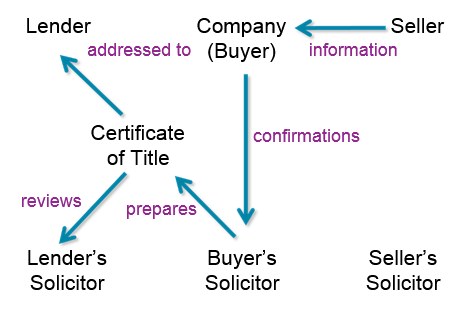
\includegraphics{C:/Users/shiva/Filen/MEGA/LegalPracticeCourse/certificate-of-title.png}

\hypertarget{timing-1}{%
\subsubsection{Timing}\label{timing-1}}

Modern practice is for title to be deduced and investigated before
exchange of contracts, and\\
for any issues that arise from this process to be resolved before that
point. If this is the case, as\\
the buyer will already have had his opportunity to raise any queries and
will have entered into\\
the contract with full knowledge of what the title contains, it is usual
to find that the contract\\
will contain a provision preventing the buyer raising requisitions on
some or all aspects of the\\
title once exchange has taken place (see SC 4.2.1 and SCPC 7.2.1).

If, exceptionally, title is deduced after exchange, the contract will
usually contain a timetable for the raising of, and responding to,
requisitions (see SC 4.3 and SCPC 7.3).

\hypertarget{investigation}{%
\subsubsection{Investigation}\label{investigation}}

Elements of buyer's investigation:

\begin{enumerate}
\tightlist
\item
  Title will be deduced by the seller in the form of official copies of
  the entries on the register and the title plan, and so, first, a
  thorough examination of these must be undertaken.

  \begin{itemize}
  \tightlist
  \item
    Property register

    \begin{itemize}
    \tightlist
    \item
      Does the description of the land agree with the contract
      description?
    \item
      Does the title number match the one given in the contract?
    \item
      Is the estate freehold or leasehold? Does this accord with
      expectations from the contract
    \item
      Which easements are enjoyed by the property? Do these match the
      needs of the client?
    \end{itemize}
  \item
    Proprietorship register

    \begin{itemize}
    \tightlist
    \item
      Is the class of title correct?
    \item
      Is the seller the registered proprietor? If not, who has the
      ability to transfer the land?
    \item
      Are there any other entries? What is their effect?
    \end{itemize}
  \item
    Charges register

    \begin{itemize}
    \tightlist
    \item
      Are there any incumbrances?
    \item
      How do these affect the buyer?
    \item
      Which of them will be removed or discharged on completion?
    \item
      Have you agreed in the contract to buy subject to the incumbrances
      which remain?
    \end{itemize}
  \item
    Title plan

    \begin{itemize}
    \tightlist
    \item
      Is the land being bought included within the title?
    \item
      Are there any colourings/hatchings which may indicate rights of
      way, the extent of covenants or land which has been removed from
      the title?
    \end{itemize}
  \end{itemize}
\item
  Investigations to discover if there are any overriding interests
  affecting the property.
\item
  Certain checks before completion to update the information revealed
  and to ensure that no changes have taken place since the investigation
  of title was carried out.
\end{enumerate}

\hypertarget{common-title-problems}{%
\subsection{Common Title Problems}\label{common-title-problems}}

See Common Title Problems.

\hypertarget{raising-requisitions}{%
\subsection{Raising Requisitions}\label{raising-requisitions}}

If the buyer's solicitor's investigation of title reveals any problem
then the buyer should raise a `requisition on title' of the seller's
solicitor.

\begin{env-68b88379-d4cc-4b35-9b80-2115e064fa9f}

Definition

A requisition is a question asked about the problem which requires a
remedy from the seller.

\end{env-68b88379-d4cc-4b35-9b80-2115e064fa9f}

If the seller ultimately cannot show good title then the buyer may
consider whether defective title indemnity insurance is available
(perhaps at the seller's cost) in order to protect him should he decide
to proceed and accept the defect.

Standard Condition 4.3.1 (SCPC 7.3.1) requires the buyer to raise
requisitions within six working days of the later of exchange of
contracts or the delivery of the epitome.

It is usual in modern practice for the title to be deduced prior to
exchange (see 14.2).

MERMAID1

\hypertarget{common-title-problems-1}{%
\section{Common Title Problems}\label{common-title-problems-1}}

\hypertarget{trustees-of-land}{%
\subsection{Trustees of Land}\label{trustees-of-land}}

In registered land, a restriction may be entered on the proprietorship
register which will indicate to the buyer what must be done to overreach
the beneficiaries' interests. Provided the terms of the restriction are
complied with, the buyer will get good title. In all cases, the
disposition must be made by all the trustees, being at least two in
number, or a trust corporation.

\hypertarget{appointing-further-trustee}{%
\subsubsection{Appointing Further
Trustee}\label{appointing-further-trustee}}

\begin{itemize}
\tightlist
\item
  If there is only one trustee then the buyer must insist that a second
  trustee is appointed in order to overreach the interests of the
  beneficiaries (see Overreaching).
\item
  The appointment will usually be made by the surviving trustee
  (although the trust deed can confer the power of appointment on
  someone else).
\end{itemize}

\hypertarget{options}{%
\paragraph{Options}\label{options}}

\begin{enumerate}
\tightlist
\item
  The appointment can be made prior to the contract for sale being
  entered into.

  \begin{itemize}
  \tightlist
  \item
    The new trustee will thus be a party to the contract and bound by
    its terms.
  \item
    Particularly useful where the new trustee is also in occupation of
    the property.
  \end{itemize}
\item
  The sole trustee can enter into the contract on his own and then
  appoint a further trustee prior to completion, to receive the purchase
  price and thus ensure overreaching takes place.

  \begin{itemize}
  \tightlist
  \item
    A special condition can be included in the contract requiring the
    seller to appoint the further trustee
  \item
    Note, the seller would be under an obligation to do so anyway in
    order to comply with the duty to make good title.
  \end{itemize}
\end{enumerate}

\hypertarget{conveyance-by-trustees-to-themselves}{%
\subsubsection{Conveyance by Trustees to
Themselves}\label{conveyance-by-trustees-to-themselves}}

\begin{env-a1c35d52-c355-4524-93c6-325e9133bd60}

Action

In the case of a disposal by trustees or personal representatives to one
of themselves, enquiry must be made into the circumstances of the
transaction because, on the face of it, such a disposal is in breach of
trust and is voidable by the beneficiaries.

\end{env-a1c35d52-c355-4524-93c6-325e9133bd60}

\hypertarget{exceptions}{%
\paragraph{Exceptions}\label{exceptions}}

\begin{enumerate}
\tightlist
\item
  there is proof of a pre-existing contract in favour of the trustee or
  personal representative;
\item
  the personal representative was a beneficiary under the will or
  intestacy of the deceased;
\item
  the consent of all the legally competent (i.e., adult and sane)
  beneficiaries was obtained to the transaction;
\item
  the conveyance was made under an order of the court;
\item
  the transaction was sanctioned by the trust instrument.
\end{enumerate}

\hypertarget{personal-representatives}{%
\subsection{Personal Representatives}\label{personal-representatives}}

Personal representatives enjoy the same wide powers as trustees of land.

\begin{longtable}[]{@{}ll@{}}
\toprule()
Number of personal representatives & Consequence \\
\midrule()
\endhead
{\(1\)} & Has all the powers of two or more personal representatives,
and consequently (unlike a sole individual trustee) can convey the land
on her own and give a valid receipt for the proceeds of sale. \\
{\(> 1\)} & All personal representatives must join in the assent or
conveyance. \\
\bottomrule()
\end{longtable}

\begin{env-a1c35d52-c355-4524-93c6-325e9133bd60}

Action

A buyer must therefore call for the grant to see who has or have been
appointed as personal representative(s), and must insist that all the
personal representatives named in the grant join in the assent or
conveyance, or call for evidence of the death of any personal
representative who will not be a party to it.

\end{env-a1c35d52-c355-4524-93c6-325e9133bd60}

\hypertarget{registering-as-proprietors}{%
\subsubsection{Registering as
Proprietors}\label{registering-as-proprietors}}

\begin{itemize}
\tightlist
\item
  On production of the grant of probate, personal representatives
  \textbf{may} become registered as proprietors of the land

  \begin{itemize}
  \tightlist
  \item
    Buyer purchases registered land as normal.
  \item
    Rare, unless holding property for some time (e.g., for a minor)
  \end{itemize}
\item
  Grant of probate is proof of PR's authority to deal with the land.

  \begin{itemize}
  \tightlist
  \item
    Buyer takes a transfer from all the proving personal representatives
    and submits an office copy or certified copy of the grant with his
    application for registration to obtain a good title.
  \item
    An assent made by personal representatives to a beneficiary must be
    in the form prescribed under the Land Registration Rules 2003 (SI
    2003/1417).
  \end{itemize}
\end{itemize}

\hypertarget{co-ownership}{%
\subsection{Co-ownership}\label{co-ownership}}

See Co-ownership. Practical points:

\hypertarget{tenants-in-common}{%
\subsubsection{Tenants in Common}\label{tenants-in-common}}

Restriction entered on proprietorship register:

\begin{quote}
``No disposition by a sole proprietor of the registered estate (except a
trust corporation) under which capital money arises is to be registered
unless authorised by an order of the court.''
\end{quote}

If in the death of one or more co-owners there is only one surviving
trustee (and you have death certificates to prove), two options:

\begin{enumerate}
\tightlist
\item
  Comply with the restriction, which ensures a second trustee is
  appointed to join with the survivor in the transfer. Preferred and
  safest way.
\item
  Have the restriction removed because the seller can prove they are
  solely and beneficially entitled to the whole legal and equitable
  interest in the land.
\end{enumerate}

\hypertarget{joint-tenants}{%
\subsubsection{Joint Tenants}\label{joint-tenants}}

If the co-owners are joint tenants in equity, \textbf{no restriction is
placed on the register} and a buyer may generally deal safely with the
survivor alone on proof of the death of the deceased co-owner.

It is possible that the equitable joint tenancy could have been severed,
but in the absence of a restriction, only if the beneficiary of the
deceased has an overriding interest under the LRA 2002 by virtue of
being in occupation of the property will a problem arise. Conduct
searches and enquiries to check.

\hypertarget{disposing-lenders}{%
\subsection{Disposing Lenders}\label{disposing-lenders}}

See Mortgages.

s 101 LPA 1925: gives a power to sell the legal estate vested in the
borrower, subject to prior incumbrances but discharged from subsequent
ones, to every lender whose mortgage is made by deed (unless explicitly
excluded).

Only the proprietor of a registered charge has a power of sale. When a
property is sold by a lender, the buyer takes the property free from
that and any other (secondary) mortgages.

\hypertarget{power-of-sale}{%
\subsubsection{Power of Sale}\label{power-of-sale}}

\hypertarget{arises}{%
\paragraph{Arises}\label{arises}}

\href{https://www.legislation.gov.uk/ukpga/Geo5/15-16/20/section/101}{LPA
1925, s 101(1)(i)}: The power of sale arises when the mortgage money
becomes due under the mortgage, i.e., on the legal date for redemption
(usually early).

\hypertarget{exercisable}{%
\paragraph{Exercisable}\label{exercisable}}

The power becomes exercisable by the lender only as provided for in the
mortgage deed, or when one of the events specified in
\href{https://www.legislation.gov.uk/ukpga/Geo5/15-16/20/section/103}{s
103 LPA 1925} has occurred. These events are:

\begin{enumerate}
\tightlist
\item
  a demand has been made for the principal sum outstanding on the
  mortgage and this demand is unpaid for three months; or
\item
  any interest due under the mortgage is in arrears for two months; or
\item
  there is breach of any other covenant in the mortgage.
\end{enumerate}

\hypertarget{discharged-mortgages}{%
\subsection{Discharged Mortgages}\label{discharged-mortgages}}

\begin{itemize}
\tightlist
\item
  A mortgage over registered land which has been discharged will be
  deleted from the charges register of the title and is thus of no
  further concern to the buyer.
\item
  As far as the seller's existing mortgage is concerned, the buyer
  should raise a requisition requiring this to be removed on or before
  completion.
\item
  Discharge of a mortgage of registered land is effected by filing a
  completed Form DS1 at Land Registry or by use of the ED or e-DS1
  system.
\end{itemize}

\hypertarget{attorneys}{%
\subsection{Attorneys}\label{attorneys}}

\hypertarget{powers-of-attorney}{%
\subsubsection{Powers of Attorney}\label{powers-of-attorney}}

\begin{env-68b88379-d4cc-4b35-9b80-2115e064fa9f}

Definition

A power of attorney is a deed under which the donor appoints someone
(the attorney or donee) to carry out certain actions on their behalf.

\end{env-68b88379-d4cc-4b35-9b80-2115e064fa9f}

\hypertarget{types-of-power}{%
\subsubsection{Types of Power}\label{types-of-power}}

\begin{longtable}[]{@{}ll@{}}
\toprule()
Power & Description \\
\midrule()
\endhead
General power & s 10 of the Powers of Attorney Act 1971: entitles the
attorney to deal with all of the donor's assets \\
Special power & Permits the attorney to deal only with certain specified
assets or categories of assets \\
Trustee power & Used where property is held on trust \\
Enduring power & Enduring Powers of Attorney Act 1985: endures through
the donor's mental incapacity \\
Lasting power & Replaced enduring power (01/10/2007) \\
\bottomrule()
\end{longtable}

\hypertarget{revocation}{%
\subsubsection{Revocation}\label{revocation}}

Power of attorney may be revoked expressly by the donor, or will be
revoked automatically on the donor's death, mental incapacity or
bankruptcy. Once registered, enduring powers are irrevocable except by
order of the court.

A person who buys from an attorney (and subsequent buyers) will get good
title if the power:

\begin{enumerate}
\tightlist
\item
  authorises the transaction which is to take place between the attorney
  and the buyer; and
\item
  is valid and subsisting at the date of completion of the transaction.
\end{enumerate}

\hypertarget{buyer-protection}{%
\subsubsection{Buyer Protection}\label{buyer-protection}}

The buyer is given protection through the Powers of Attorney Act 1971:

\hypertarget{copy-of-power}{%
\paragraph{Copy of Power}\label{copy-of-power}}

Buyer entitled to a certified copy of the power of attorney affecting
the title--Land Registry will require a copy before registering a
disposition. Buyer should check terms of the power to ensure the
transaction was authorised.

\hypertarget{general-special-and-trustee-powers}{%
\paragraph{General, Special and Trustee
Powers}\label{general-special-and-trustee-powers}}

A person who deals with an attorney holding these types of powers of
attorney will take good title, provided he acquires in good faith
without knowledge of the revocation of the power:

\begin{env-b1feafbb-b990-4f84-956e-67a6473913ab}

s 5(2) Powers of Attorney Act 1971

Where a power of attorney has been revoked and a person, without
knowledge of the revocation, deals with the donee of the power, the
transaction between them shall, in favour of that person, be as valid as
if the power had then been in existence.

\end{env-b1feafbb-b990-4f84-956e-67a6473913ab}

Death revokes such a power.

\begin{env-b1feafbb-b990-4f84-956e-67a6473913ab}

s 5(4) Powers of Attorney Act 1971

Where the interest of a purchaser depends on whether a transaction
between the donee of a power of attorney and another person was valid by
virtue of subsection (2) of this section, it shall be conclusively
presumed in favour of the purchaser that that person did not at the
material time know of the revocation of the power if---

\begin{itemize}
\tightlist
\item
  (a) the transaction between that person and the donee was completed
  within twelve months of the date on which the power came into
  operation; or
\item
  (b) that person makes a statutory declaration, before or within three
  months after the completion of the purchase, that he did not at the
  material time know of the revocation of the power.
\end{itemize}

\end{env-b1feafbb-b990-4f84-956e-67a6473913ab}

\hypertarget{enduring-powers}{%
\paragraph{Enduring Powers}\label{enduring-powers}}

\begin{env-68b88379-d4cc-4b35-9b80-2115e064fa9f}

Definition

An enduring power of attorney is one made under the Enduring Powers of
Attorney Act 1985. This Act has been repealed and enduring powers are
now governed by provisions contained in Sch 4 to the Mental Capacity Act
2005.

\end{env-68b88379-d4cc-4b35-9b80-2115e064fa9f}

Until the incapacity of the donor, the power takes effect as an ordinary
power and the Mental Capacity Act contains provisions to protect buyers
which are similar to those outlined above. On the incapacity of the
donor, the attorney's authority to act becomes limited to such acts as
are necessary for the protection of the donor and his estate until such
time as the power is registered with the Office of the Public Guardian.

\begin{env-a1c35d52-c355-4524-93c6-325e9133bd60}

Action

Where a person is buying from an attorney who holds an enduring power,
he should make a search at the Office of the Public Guardian to ensure
that no application for registration of the power is pending. If an
application is pending, this would suggest mental incapacity on the part
of the donor.

\end{env-a1c35d52-c355-4524-93c6-325e9133bd60}

\hypertarget{lasting-powers}{%
\paragraph{Lasting Powers}\label{lasting-powers}}

\begin{env-68b88379-d4cc-4b35-9b80-2115e064fa9f}

Definition

The Mental Capacity Act 2005 (in force 1 October 2007) replaced enduring
powers with a new form of power called a lasting power. Lasting powers
give an attorney power to deal with the donor's personal welfare and/or
his property and affairs, including authority to deal with such matters
when the donor no longer has capacity.

\end{env-68b88379-d4cc-4b35-9b80-2115e064fa9f}

The lasting power is required to be in a prescribed form but, unlike
enduring powers, comes into effect only when registered with the Office
of the Public Guardian.

\begin{env-a1c35d52-c355-4524-93c6-325e9133bd60}

Action

Where the buyer is buying from an attorney who holds a lasting power, he
should obtain an office copy of the power from the Office of the Public
Guardian as evidence that the lasting power is registered with the
Office of the Public Guardian and to check that the attorney is acting
within the scope of his authority.

The buyer from the attorney will be protected unless he knew the power
was invalid (by s 14(3) of the Mental Capacity Act 2005) or was aware of
circumstances which would have terminated the attorney's authority to
act (by s 5(2) of the Powers of Attorney Act 1971).

\end{env-a1c35d52-c355-4524-93c6-325e9133bd60}

\hypertarget{trustees}{%
\paragraph{Trustees}\label{trustees}}

\begin{env-8d28ec84-dab8-490f-8d30-94b3086ae3c1}

Guidance

If one of two co-owners wishes to appoint an attorney to execute a deed
selling the land, the co-trustee cannot be appointed, as such co-trustee
will not be able to give a valid receipt. In such a case, a stranger
will need to be appointed, and this rule cannot be evaded by using an
enduring power.

\end{env-8d28ec84-dab8-490f-8d30-94b3086ae3c1}

\hypertarget{transactions-at-an-undervalue}{%
\subsection{Transactions at an
Undervalue}\label{transactions-at-an-undervalue}}

\begin{env-6551cd31-4c34-4de5-9b70-48dd453ea5fd}

Warning

Where in the chain of title there is a transaction for no consideration
or at an undervalue, care needs to be exercised, since the transaction
could be set aside under the Insolvency Act 1986.

\end{env-6551cd31-4c34-4de5-9b70-48dd453ea5fd}

\begin{longtable}[]{@{}lll@{}}
\toprule()
Party & Rule & Statute \\
\midrule()
\endhead
Individual & A transaction at an undervalue by an individual within the
five years immediately preceding the current transaction may be set
aside by the trustee in bankruptcy if the donor is made bankrupt & s 339
IA 1986 \\
Company & If a transaction at an undervalue was made by a company within
the two years preceding the date of the current transaction, it may be
set aside by the liquidator on the company's subsequent insolvency & s
238 IA 1986 \\
\bottomrule()
\end{longtable}

\hypertarget{buyer-defences}{%
\subsubsection{Buyer Defences}\label{buyer-defences}}

\begin{env-8e984a52-6a47-430d-9005-822950744b1a}

Note

The basic principle is that a subsequent buyer is protected, provided
that he has acquired in good faith and for value from a person other
than the insolvent company or bankrupt individual (Insolvency Act 1986,
s 241(2)(a) and s 342(2)(a)).

\end{env-8e984a52-6a47-430d-9005-822950744b1a}

See Business Law and Practice/Insolvency/Voidable Transactions
\textgreater{} Sanctions above for details on presumption of good faith.
Remember, connected person includes directors, shadow directors and
associates. Associate defined widely in s 435 IA 1986 to include a
person's spouse or ex-spouse, members of his family and his spouse's
family, his partner and his partner's family, and his employees.

\begin{env-a1c35d52-c355-4524-93c6-325e9133bd60}

Action

\begin{itemize}
\tightlist
\item
  Registration of bankruptcy proceedings will amount to notice, so a
  buyer will need to make a bankruptcy search against the individual
  making the transaction at an undervalue not for the period of that
  person's ownership, but for a period of five years from the date of
  the transaction at an undervalue.
\item
  In the case of companies, the relevant time is 2 years.
\end{itemize}

\end{env-a1c35d52-c355-4524-93c6-325e9133bd60}

\hypertarget{registered-land}{%
\subsubsection{Registered Land}\label{registered-land}}

In the case of dispositions registered on or after 1 April 2000, the
register includes details of the price paid by the proprietor.

\begin{env-a1c35d52-c355-4524-93c6-325e9133bd60}

Action

If this appears to be nil or something of low monetary value, the
provisions of the Insolvency Act 1986 should be borne in mind.

\end{env-a1c35d52-c355-4524-93c6-325e9133bd60}

Where first registration is based on a transaction at an undervalue, a
note will be added in the proprietorship register to the effect that the
title is subject to the provisions of the Insolvency Act 1986.

Some lenders are reluctant to lend on property where there has been a
transaction at an undervalue within the past two years (companies) or
five years (individuals), unless an \textbf{insurance} policy is
obtained covering the possibility of the donor's insolvency within these
periods.

\hypertarget{restrictive-covenants}{%
\subsection{Restrictive Covenants}\label{restrictive-covenants}}

Instructions may reveal that the buyer's intended use of the property
after completion will cause a breach of existing covenants.

\begin{enumerate}
\tightlist
\item
  Check whether the covenant is registered (usually is)
\item
  Look at the wording of the covenant to see whether it has been annexed
  to the land and is prima facie binding.
\item
  Consider whether it is possible to obtain an insurance policy to cover
  liability for future breaches of covenant. Insurance company will need
  details of the covenant, local area, any steps taken etc.
\end{enumerate}

\hypertarget{ending-freehold-covenants}{%
\subsubsection{Ending Freehold
Covenants}\label{ending-freehold-covenants}}

The methods by which a freehold covenant can be brought to an end are
discharge, modification and release.

\hypertarget{problem-with-old-covenants}{%
\paragraph{Problem with Old
Covenants}\label{problem-with-old-covenants}}

Restrictive covenants, once validly granted, last forever. Over time,
these can become obsolete and can unduly restrict the use of the
servient land.

\begin{env-c75278ec-0f81-4db3-97b1-0452147ba646}

Example

A covenant not to build on land might have benefitted the dominant
tenement whilst that land was used for residential purposes, but no
longer does if the dominant land is now a factory.

\end{env-c75278ec-0f81-4db3-97b1-0452147ba646}

There are various ways in which a covenant can be discharged or
modified. Discharge if a covenant means that it is no longer valid.

Modification of a covenant means that the scope of the covenant is
altered, but it is not completely invalidated.

\hypertarget{methods-of-dischargingmodifying-covenants}{%
\paragraph{Methods of discharging/modifying
Covenants}\label{methods-of-dischargingmodifying-covenants}}

A covenant will be automatically be discharged if the same person
becomes the owner of both the dominant and servient land: Re Tiltwood,
Sussex {[}1978{]} Ch 269.

This is known as merger. A dominant owner may expressly agree to
discharge the covenant and will enter into a formal release of covenant,
usually in return for a payment.

The release must be made by deed. Alternatively, the dominant owner may
impliedly agree to discharge the covenant by doing nothing when the
covenant is being breached openly.

\hypertarget{statutory-discharge-or-modification-of-covenants}{%
\paragraph{Statutory Discharge or Modification of
Covenants}\label{statutory-discharge-or-modification-of-covenants}}

The dominant owner could hold the servient owner to ransom by asking for
a large sum of money to discharge an obsolete covenant.

To avoid this, the servient owner can apply to the Tribunals
\textgreater{} Upper Tribunal (Lands Chamber) for the discharge or
modification of any covenant.

\href{https://www.legislation.gov.uk/ukpga/Geo5/15-16/20/section/84}{Law
of Property Act 1925, s 84(1)} gives the Lands Chamber the power `wholly
or partially to discharge or modify any\ldots{} restriction'.

\begin{env-6551cd31-4c34-4de5-9b70-48dd453ea5fd}

Warning

This provision only applies to restrictive covenants.

\end{env-6551cd31-4c34-4de5-9b70-48dd453ea5fd}

\begin{env-b1feafbb-b990-4f84-956e-67a6473913ab}

\href{https://www.legislation.gov.uk/ukpga/Geo5/15-16/20/section/84}{LPA
1925, s 84(1)(a)}

A servient owner may apply to the tribunal for a declaration to
discharge or modify a covenant on the basis that the covenant has become
obsolete due to changes in the character of the property or
neighbourhood.

\end{env-b1feafbb-b990-4f84-956e-67a6473913ab}

\begin{env-c75278ec-0f81-4db3-97b1-0452147ba646}

Example

A covenant to use property only as a residence may be obsolete if the
surrounding area is now business, retail of mixed use.

\end{env-c75278ec-0f81-4db3-97b1-0452147ba646}

\href{https://www.legislation.gov.uk/ukpga/Geo5/15-16/20/section/84}{s
84(1)(aa)} enables an application to be made on the basis that the
covenant impedes reasonable use of the servient land. The applicant must
show either that the covenant confers no practical value, or that it is
contrary to public interest.

The tribunal must be satisfied that financial compensation would be
adequate for the dominant owner.

\begin{env-c75278ec-0f81-4db3-97b1-0452147ba646}

Example

A covenant restricting the density of houses on a plot may confer no
practical value on the dominant land if that land is itself densely
developed.

\end{env-c75278ec-0f81-4db3-97b1-0452147ba646}

S 84(1)(b) applies where the dominant owners have agreed, expressly or
impliedly, to discharge.

\begin{env-c75278ec-0f81-4db3-97b1-0452147ba646}

Example

An application here may be appropriate where the parties have expressly
agreed a release in principle, or where the dominant owner has tolerated
a long-term breach. In this instance, the tribunal will decide the level
of compensation to be paid, thereby preventing the dominant owner
holding the servient owner to ransom.

\end{env-c75278ec-0f81-4db3-97b1-0452147ba646}

S 84(1)(c) enables an application to be made where discharge if a
covenant will not 'injure' the dominant owners.

This provision means that the tribunal can override spurious or
frivolous objections.

However, the tribunal has a balancing act to do: on the one hand it will
be wary of discharging covenants on this basis simply because discharge
will not injure the current dominant owner. On the other hand it will
have regard to social and economic concerns: the wider public interest
rather than the interest of one particular dominant owner.

\hypertarget{insurance}{%
\subsubsection{Insurance}\label{insurance}}

If a policy is issued, it is normally a single premium policy (a single
sum is paid on the issue of the policy). The benefit of the policy may
be passed on to successors in title. The buyer's lender should be
consulted about the proposed breach of covenant and his approval
obtained to the terms of the insurance policy.

\begin{env-633e2c1a-5d4f-4828-b85f-3631067ba172}

Danger

In arranging or advising on such a policy, the solicitor is carrying out
a `regulated activity' for the purposes of the FSMA 2000. Ensure you
fall within the professional firms exemption to avoid committing a
criminal offence.

\end{env-633e2c1a-5d4f-4828-b85f-3631067ba172}

\hypertarget{other-methods}{%
\subsubsection{Other Methods}\label{other-methods}}

To be used only if insurance is not possible.

\begin{itemize}
\tightlist
\item
  Approach the person with the benefit of the covenant.

  \begin{itemize}
  \tightlist
  \item
    Often they may accept payment for release from the covenant.
  \item
    But there might be multiple parties with the benefit of the covenant
  \item
    By putting the benefitting party on notice, makes it almost
    impossible to get insurance.
  \end{itemize}
\item
  Apply to Upper Tribunal (Lands Chamber)

  \begin{itemize}
  \tightlist
  \item
    Has power in certain circumstances under the LPA 1925, s 84 to grant
    a modification or discharge of a restrictive covenant.
  \end{itemize}
\end{itemize}

\hypertarget{competition-legislation}{%
\subsubsection{Competition Legislation}\label{competition-legislation}}

\hypertarget{competition-act-1998}{%
\paragraph{Competition Act 1998}\label{competition-act-1998}}

\begin{itemize}
\tightlist
\item
  This prohibits any agreement which may affect trade within the UK and
  which prevents, restricts or distorts competition within the UK.
\item
  Since April 2011 this prohibition has applied to land agreements,
  which include transfers of freehold and leasehold interests together
  with leases themselves.
\item
  It only applies to agreements between businesses
\item
  It is retrospective, thus the date of the covenant is irrelevant.
\item
  It is not possible to exclude the Act.
\end{itemize}

\hypertarget{prohibited-restrictions}{%
\paragraph{Prohibited Restrictions}\label{prohibited-restrictions}}

Unless the covenant has an `appreciable effect' on the market affected
by the\\
agreement, it will not fall within the competition legislation. Whether
such provisions have an appreciable effect depends on a number of
factors, including the scope of the relevant market and the degree of
market power of the parties.

\hypertarget{consequences}{%
\paragraph{Consequences}\label{consequences}}

\begin{itemize}
\tightlist
\item
  Fines of up to 10\% of a firm's worldwide turnover
\item
  Agreement containing a prohibited restriction void and unenforceable
  (though a court may consider it possible to sever the prohibited
  restriction and let other terms of the agreement remain valid).
\end{itemize}

\hypertarget{groceries}{%
\paragraph{Groceries}\label{groceries}}

Certain land agreements in connection with grocery retailing activities
are subject to\\
additional control under the Groceries Market Investigation (Controlled
Land) Order 2010 (the `Controlled Land Order').

\hypertarget{positive-covenants}{%
\subsection{Positive Covenants}\label{positive-covenants}}

The burden (the obligation to observe a covenant) does not generally
bind successors in title of freehold land where a covenant is positive
in nature. There is one anomalous exception to this principle, a fencing
"easement".

A positive covenant may be enforced at law even though the covenantor
owns no estate of any kind in land. The common law only requires that
the covenantee must hold an estate in land to which the benefit of an
enforceable covenant can accrue.

Although the burden of a positive covenant does not run with the land,
there are various workarounds which can be adopted to ensure a similar
outcome.

\hypertarget{passing-burden}{%
\subsubsection{Passing Burden}\label{passing-burden}}

\begin{itemize}
\tightlist
\item
  Chain of indemnity

  \begin{itemize}
  \tightlist
  \item
    Although a positive obligation is not directly enforceable against a
    successor in title, it may be indirectly enforceable through
    indemnities given by a buyer to the previous owner.
  \item
    But chain only as strong as its weakest link
  \item
    Only damages can be obtained, not injunction etc.
  \end{itemize}
\item
  Compulsory renewed covenants supported with a restriction

  \begin{itemize}
  \tightlist
  \item
    Most common way of making the burden of positive covenants run.
  \item
    The transferee gives a binding obligation to compel its own
    successor to:

    \begin{itemize}
    \tightlist
    \item
      Enter into a direct covenant with the dominant owner at the date
      of the new covenant, in the same terms as the initial positive
      covenant.
    \item
      Impose a further obligation to provide a direct covenant in
      similar terms on its successor.
    \end{itemize}
  \item
    Risk: the covenantor could transfer the land without complying with
    its obligation to obtain a further covenant from the transferee.
    Breach of contract remedies will be inadequate.
  \item
    Common practice to ensure compliance by adding an appropriately
    worded restriction on the servient landowner's title: ``no
    disposition of the land in that title should be registered without a
    certificate signed by a conveyancer confirming that the requirement
    to provide a new deed of covenant has been met''.
  \item
    But inappropriate where lots of people benefit from the covenants,
    in particular where there are numerous plots of dominant land.
  \end{itemize}
\item
  Right of entry annexed to an estate rentcharge

  \begin{itemize}
  \tightlist
  \item
    To secure the performance of positive covenants, the owner of the
    land may reserve a rentcharge to which it annexes a right of entry.
  \item
    A rentcharge is ``any annual or other periodic sum of money charged
    on or issuing out of land'', otherwise than under a lease or
    mortgage".
  \item
    An estate rentcharge can be used to enforce a positive obligation,
    because the chargor takes a legal right of entry (i.e., possession)
    in the event of default.
  \item
    The right of entry may be exercised not only for failure to pay the
    rentcharge, but also for breach of the covenant, subject to the
    court providing relief against forfeiture.
  \item
    Draconian for buyers
  \item
    The rentcharge may be for a nominal amount and serves as a peg on
    which to hang the enforcement of the covenant.
  \end{itemize}
\item
  Benefit and burden rule

  \begin{itemize}
  \tightlist
  \item
    See section below.
  \item
    So be careful about relying on Halsall v Brizell {[}1957{]} Ch 169
    in practice: there is a risk the courts will not recognise a
    condition precedent to an obligation to repair/ maintain something.
  \end{itemize}
\item
  Freehold right of re-entry

  \begin{itemize}
  \tightlist
  \item
    The seller transfers the property to the buyer, but retains an
    express (equitable) right of re-entry, under which the property will
    revert to the seller if the positive covenant is not performed.
  \item
    As the right of re-entry is an equitable interest, it should be
    protected by a notice registered against the buyer's title to the
    property.
  \item
    Draconian and rarely used in practice.
  \item
    May make borrowing problematic
  \end{itemize}
\item
  Use of leasehold title

  \begin{itemize}
  \tightlist
  \item
    The burden of a positive covenant may run with a leasehold estate.
  \item
    s 153 LPA 1925: grants a right to enfranchise (expressed as a right
    to enlarge the term of the lease into a fee simple).
  \item
    Where a lease may be enlarged into a freehold, section 153 provides
    that it will be subject to the same covenants, obligations and
    provisions which burdened the lease.
  \item
    Untested, complicated.
  \end{itemize}
\end{itemize}

\hypertarget{mutual-benefit-and-burden}{%
\paragraph{Mutual Benefit and Burden}\label{mutual-benefit-and-burden}}

Halsall v Brizell {[}1957{]} Ch 169 gives a limited exception to the
general rule, enabling the burden of a covenant to pass to a successor
covenantor at common law. It is known as the \textbf{`mutual benefit and
burden' rule}, and applies where the covenantee grants to the covenantor
a benefit in the nature of an easement, and imposes a connected burden.

For example, in the transfer deed selling part of a piece of land, a
covenantee grants the covenantor a right to park on the covenantee's
land. In the same deed, the covenantor covenants to contribute to the
cost of maintaining the parking area.

In a case like this, a successor covenantor cannot take the benefit of
parking but avoid payment by relying on the basic common law rule of the
burden not passing.

\hypertarget{refinements}{%
\subparagraph{Refinements}\label{refinements}}

The rules has been refined in subsequent cases:

\begin{longtable}[]{@{}ll@{}}
\toprule()
Case & Ratio \\
\midrule()
\endhead
Rhone v Stephens {[}1994{]} 2 AC 310 & There must be a clear link
between the burden and the benefit. There is no general principle that
someone who takes a benefit under a deed must submit to any burden which
it imposes. \\
Thamesmead Town Ltd v Allotey (1998) 3 EGLR 97 & There must be a genuine
choice as to whether or not to take the benefit. This choice can be
theoretical. The condition of discharging the covenanted burden must be
relevant to the exercise of the right (more than incidental). \\
Davies v Jones {[}2009{]} EWCA Civ 1164 & The benefit and burden must
have been conferred in the same transaction. \\
\bottomrule()
\end{longtable}

\hypertarget{grant-of-long-lease}{%
\subparagraph{Grant of Long Lease}\label{grant-of-long-lease}}

One way of side-stepping the rule that the burden of a freehold covenant
will not pass to a successor covenantor is to dispose of the land by way
of long lease.

All covenants in leases except personal ones are enforceable by and
against successors in title via the doctrine of privity of estate.

\hypertarget{commonhold-development}{%
\subparagraph{Commonhold Development}\label{commonhold-development}}

Commonhold is a way of holding land in units such as blocks of flats.
Each unit owner has obligations, such as contributing towards the
maintenance of each unit. The rights and obligations attach by statute
(\href{https://www.legislation.gov.uk/ukpga/2002/15/contents}{Commonhold
and Leasehold Reform Act 2002}) to each unit, so all obligations are
enforceable against all unit holders at all times.

Unfortunately, commonhold has not proved a popular way of holding land.

\hypertarget{restriction-s-40-lra-2002}{%
\subparagraph{Restriction: S 40 LRA
2002}\label{restriction-s-40-lra-2002}}

\begin{env-8e984a52-6a47-430d-9005-822950744b1a}

Note

This is the most commonly used way of making the burden of positive
covenants run on registered land.

\end{env-8e984a52-6a47-430d-9005-822950744b1a}

A covenantee can put a restriction on the \textbf{proprietorship
register of the burdened land}. This states that no transfer of the
burdened land can be registered without the consent of the covenantee.

As a condition of giving consent to the transaction, the covenantee
takes a direct covenant from the purchaser of the burdened land.

In the new covenant, the new owner promises to observe the covenants in
the original transfer. This creates a new privity of contract between
the covenantee and purchaser, enabling direct enforcement of the
covenants.

\hypertarget{other-methods-1}{%
\subparagraph{Other Methods}\label{other-methods-1}}

\begin{itemize}
\tightlist
\item
  Reserving a rentcharge annexed to a right of entry
\item
  Reserving a freehold right of entry
\item
  Less commonly used.
\end{itemize}

\hypertarget{passing-benefit}{%
\subsubsection{Passing Benefit}\label{passing-benefit}}

The original covenantee can enforce a covenant as a matter of contract
law. If the dominant land is sold, the successor covenantee must show
that the benefit has passed to it at common law.

This enables the successor covenantee to enforce the covenant either
against the original covenantor, or (in limited circumstances) against
the successor covenantor.

There are two ways the benefit can pass at common law:

\hypertarget{express-assignment}{%
\paragraph{Express Assignment}\label{express-assignment}}

Under normal contractual principles, the benefit of a covenant can be
expressly assigned to a successor.

\href{https://www.legislation.gov.uk/ukpga/Geo5/15-16/20/section/136}{LPA
1925, s 136} requires the assignment must be in writing and express
notice of the assignment must be given to the covenantor. This is to
ensure that the covenantor realises that a new person is in a position
to enforce the covenant.

\hypertarget{implied-assignment}{%
\paragraph{Implied Assignment}\label{implied-assignment}}

Where there is no express assignment, the benefit of a covenant may pass
to a successor covenantee if certain conditions are met. This involves
the benefit automatically passing every time the land is transferred, as
long as the conditions are met.

\begin{env-40671eed-0836-415a-96f9-b6b8ee9a8b3f}

Implied assignment

The conditions of implied assignment are set out in P\&A Swift
Investments Ltd v Combined English Stores Group plc {[}1989{]} AC 632:

\begin{enumerate}
\tightlist
\item
  The covenant must touch and concern the land
\item
  There must have been an intention that the benefit should run with the
  dominant land
\item
  The original covenantee must have a legal estate in the dominant land
\item
  The successor covenantee must hold a legal estate in the dominant land
\end{enumerate}

\end{env-40671eed-0836-415a-96f9-b6b8ee9a8b3f}

\hypertarget{the-covenant-must-touch-and-concern-the-land}{%
\paragraph{The Covenant Must Touch and Concern the
Land}\label{the-covenant-must-touch-and-concern-the-land}}

The covenant must benefit the dominant land itself, it must affect the
nature, quality, use or value of the land. It must not be expressed to
be personal and should only benefit the dominant owner for the time
being, so that, if separated from the land, it ceases to be of any
advantage to them.

\begin{env-c75278ec-0f81-4db3-97b1-0452147ba646}

Example

A covenant to maintain a house on the burdened land does touch and
concern the dominant land as it preserves the quality of the environment
and therefore the value of the dominant land.

\end{env-c75278ec-0f81-4db3-97b1-0452147ba646}

\hypertarget{intention-that-benefit-runs-with-dominant-land}{%
\paragraph{Intention That Benefit Runs with Dominant
Land}\label{intention-that-benefit-runs-with-dominant-land}}

Intention of the parties can be shown expressly or impliedly through
statute.

If there is no express intention,
\href{https://www.legislation.gov.uk/ukpga/Geo5/15-16/20/section/78}{LPA
1925, s 78} implies an intention for the benefit to pass unless it is
expressly excluded.

\begin{env-c75278ec-0f81-4db3-97b1-0452147ba646}

Example

A covenant drafted `for the benefit of land known as 5 High Street' or
`with the covenantee and successors in title to land known as 5 High
Street' shows express intention

\end{env-c75278ec-0f81-4db3-97b1-0452147ba646}

The original covenantee must have a legal estate in the dominant land,
and the successor covenantee must hold a legal estate in the dominant
land.

The original covenantee must have owned a legal estate when the covenant
was made, and that the successor must own a legal estate at the time of
enforcement.

The legal estate does not need to be of the same nature: Smith and
Snipes Hall Farm Ltd v River Douglas Catchment Board {[}1949{]} 2 KB
500.

In that case, the original covenantee held a freehold and the successor
held a leasehold. The successor was held to be entitled to the benefit
of the covenant and could therefore enforce it.

\hypertarget{drafting-transfer}{%
\subsubsection{Drafting Transfer}\label{drafting-transfer}}

Best practice to refer to all the positive covenants together in one of
the following ways:

\begin{enumerate}
\tightlist
\item
  "the Transferee covenants with the Transferor, for the benefit of the
  Transferor's Retained Land and each and every part of it, with the
  intention of binding the Property and each and every part of it, to
  comply with the covenants set out in the sub-clauses."
\item
  "the Transferee covenants with the Transferor, for the benefit of the
  Transferor's Retained Land and each and every part of it, with the
  intention of binding the Property and each and every part of it, to
  comply with the covenants set out in Schedule {[}NUMBER{]}."
\end{enumerate}

\hypertarget{execution-of-deeds}{%
\subsection{Execution of Deeds}\label{execution-of-deeds}}

Check deeds are properly executed.

In the case of registered land, title is updated by Land Registry
whenever there is a dealing in respect of that title. As part of this
process, Land Registry will scrutinise the execution of the document
giving effect to that dealing before recording its effect on the
register.

\hypertarget{by-an-individual}{%
\subsubsection{By an Individual}\label{by-an-individual}}

\hypertarget{new-rule}{%
\paragraph{New Rule}\label{new-rule}}

The formalities for execution of a deed changed on 31 July 1990. For
deeds executed on or after 31 July 1990, the following rules apply
(\href{https://www.legislation.gov.uk/ukpga/1989/34/section/1}{s 1
LP(MP)A 1989}):

\begin{enumerate}
\tightlist
\item
  A deed must be clear on the face of the document that it is
  \textbf{intended} to be a deed

  \begin{itemize}
  \tightlist
  \item
    Satisfied by labelling the document as a deed
  \end{itemize}
\item
  The deed must be validly \textbf{executed}

  \begin{itemize}
  \tightlist
  \item
    Where the grantor (seller) is an individual, the deed must be signed
    by the seller in the presence of a witness.
  \item
    The witness needs to sign the deed to confirm that they have
    witnessed the signing of the deed by the individual entering into
    that deed. Described in statute as 'attesting' the signature.
  \item
    There is no legal requirement for a buyer to sign the deed, but in
    practice both parties tend to execute the deed.
  \end{itemize}
\item
  The deed must be \textbf{delivered}.

  \begin{itemize}
  \tightlist
  \item
    This requires an acknowledgement that a person entering into a deed
    intends to be formally bound by its provisions. In practice, this
    takes place by dating the document, which the parties' solicitors
    will do.
  \end{itemize}
\end{enumerate}

It is possible for an individual to direct another person to sign a deed
on his behalf, provided that the\\
signature is made in his presence and there are two attesting witnesses.

\hypertarget{old-rule}{%
\paragraph{Old Rule}\label{old-rule}}

The document had to be signed and sealed by its maker, and delivered as
his deed. The seal was usually only a red, self-adhesive circular piece
of paper. The delivery of the deed was a matter of intention.

\hypertarget{by-a-company}{%
\subsubsection{By a Company}\label{by-a-company}}

In the case of deeds executed by a company on or after 31 July 1990, a
document can be executed in one of three ways:

\begin{enumerate}
\tightlist
\item
  By the affixing of the company seal.

  \begin{itemize}
  \tightlist
  \item
    It must be clear on the face of the document that is intended to be
    a deed.
  \item
    If this method of execution is used, the document is deemed, in
    favour of a purchaser, to have been duly executed, provided that the
    seal purports to have been affixed in the presence of and attested
    by two members of the board of directors or a director and the
    secretary.
  \end{itemize}
\item
  By being signed by a director and the secretary, or by two directors
  of the company, provided that the document is expressed to be executed
  by the company.
\item
  A deed can be executed by being signed by a single director in the
  presence of a witness who then attests that signature (on/after
  06/04/2008 only).
\end{enumerate}

\begin{env-6551cd31-4c34-4de5-9b70-48dd453ea5fd}

Warning

Must say 'executed as a deed', 'signed as a deed' is not acceptable.

\end{env-6551cd31-4c34-4de5-9b70-48dd453ea5fd}

Must also be delivered as a deed.

\hypertarget{searches-and-enquiries}{%
\section{Searches and Enquiries}\label{searches-and-enquiries}}

\hypertarget{reasons}{%
\subsection{Reasons}\label{reasons}}

\begin{itemize}
\tightlist
\item
  Caveat emptor
\item
  When drafting the contract, the seller has only very limited duties to
  disclose matters affecting title to the property.
\item
  Buyer's solicitor must take steps to ensure the suitability of the
  property.
\item
  Failure can give rise to liability in negligence, if the buyer
  subsequently suffers loss (Cooper v Stephenson (1852) 21 LJQB 292)
\item
  Buyer must be fully advised of the information discovered and its
  implications for the proposed purchase.
\end{itemize}

\hypertarget{who}{%
\subsection{Who}\label{who}}

Buyer must make all necessary pre-conduct searches. Lender's Handbook
requires that all searches be {\(\leq 6\)} months old at the date of
completion.

\hypertarget{how}{%
\subsection{How}\label{how}}

Many searches can be undertaken electronically. Searches with the local
authority can take several weeks.

\hypertarget{what}{%
\subsection{What}\label{what}}

Standard in every transaction:

\begin{itemize}
\tightlist
\item
  Search of local land charges register
\item
  Enquiry of local authority
\item
  Pre-contract enquiries of seller
\item
  Water and drainage enquiries
\item
  Environmental search
\item
  Personal inspection.
\end{itemize}

Additional searches:

\begin{itemize}
\tightlist
\item
  Chancel repair search
\item
  Index map search
\item
  Land Charges Department search against seller's name/ previous owners'
  names for unregistered land.
\item
  Company search
\item
  Flood search
\item
  Location specific searches
\item
  Survey reports.
\end{itemize}

\hypertarget{local-land-charges-search}{%
\subsection{Local Land Charges Search}\label{local-land-charges-search}}

\begin{env-68b88379-d4cc-4b35-9b80-2115e064fa9f}

Local land charges

Financial charges or restrictions on land imposed by public authorities
under statute.

\end{env-68b88379-d4cc-4b35-9b80-2115e064fa9f}

Essential to search this in every transaction. It will be necessary to
search either a register maintained by the local authority or the land
registry, depending on the area. A fee is payable for an official
search.

Search result is given by way of certificate, digitally signed by an
officer of the council/ Land Registry (LR taking over slowly under
Infrastructure Act 2015). A fee is payable for copies of documents. The
search will reveal any entries kept under statutory obligations. Might
overlap with information from Form CON29, but should still do both to
complete due diligence.

\hypertarget{examples}{%
\subsubsection{Examples}\label{examples}}

\begin{env-c75278ec-0f81-4db3-97b1-0452147ba646}

Matters revealed by local land charges

\begin{itemize}
\tightlist
\item
  Financial charges
\item
  Tree preservation orders
\item
  Smoke control orders
\item
  Compulsory purchase orders
\item
  Planning permission granted
\item
  Restrictions on permitted development
\item
  Orders revoking/ modifying planning permissions.
\item
  Conservation area designation orders
\item
  Listed building status.
\end{itemize}

\end{env-c75278ec-0f81-4db3-97b1-0452147ba646}

For each, consider:

\begin{enumerate}
\tightlist
\item
  Significance
\item
  How it affects buyer's intended use of building.
\end{enumerate}

\hypertarget{liability}{%
\subsubsection{Liability}\label{liability}}

Where a person suffers as a result of an error in an official
certificate of search, compensation may be payable under s 10 of the
Local Land Charges Act 1975.

\hypertarget{enquiries-of-local-authority}{%
\subsection{Enquiries of Local
Authority}\label{enquiries-of-local-authority}}

\begin{itemize}
\tightlist
\item
  Submit Form CON29 to the appropriate authority (district/ London
  council).

  \begin{itemize}
  \tightlist
  \item
    CON29 relevant to every transaction.
  \end{itemize}
\item
  CON29O more specialised in nature.

  \begin{itemize}
  \tightlist
  \item
    Consider whether needed.
  \end{itemize}
\end{itemize}

CON29 will reveal:

\begin{itemize}
\tightlist
\item
  Any planning permissions granted/ refused / pending
\item
  Whether roads are public.
\item
  Any public paths or right of way
\item
  Any new roads or railways proposed near building.
\item
  Any proposals for permanently stopping up roads or footpaths.
\item
  Any proceedings for breach of building regulations
\item
  Any proposed compulsory purchase orders.
\item
  Any notice served of contaminated land.
\item
  Radon gas
\item
  Whether a property is of community value.
\end{itemize}

CON29O:

\begin{itemize}
\tightlist
\item
  Special designation area
\item
  Environmental/ pollution notices
\item
  Registration of common land/ village green.
\end{itemize}

\hypertarget{liability-1}{%
\subsubsection{Liability}\label{liability-1}}

Subject to the validity of the exclusion clause printed on the front
sheet of the search application form, a local authority could be sued in
negligence for an erroneous reply to the printed enquiries.

\hypertarget{forms-llc1-vs-con29o}{%
\subsubsection{Forms LLC1 Vs CON29/O}\label{forms-llc1-vs-con29o}}

\begin{longtable}[]{@{}llll@{}}
\toprule()
Form & Extent & Liability & Information revealed \\
\midrule()
\endhead
LLC1 & Will only reveal matters falling within the statutory definition
of a local land charge. & Negligence need not be established for
liability & Restricted to information on the register at the moment the
search is made. \\
CON29/O & Wide range of matters & Negligence must be established for
liability & May reveal information which affected property in the past,
or will do so in future. \\
\bottomrule()
\end{longtable}

\hypertarget{personal-searches}{%
\subsubsection{Personal Searches}\label{personal-searches}}

The local authority can take a few weeks to get back. Possible to
undertake a personal search with an agent if needed urgently - the agent
will personally search the offices of the appropriate local authority.
There are third party providers holding local information. Some mortgage
lenders will not accept personal searches.

\hypertarget{regulation}{%
\paragraph{Regulation}\label{regulation}}

There is a 'Search Code' monitored and enforced by the Property Codes
Compliance Board.

\hypertarget{seller-enquiries}{%
\subsection{Seller Enquiries}\label{seller-enquiries}}

Pre-contract enquiries of the seller is one of the usual searches made
in every transaction. Object is to obtain information which the seller
is not bound by law to disclose. The seller could refuse to answer - but
this would not make commercial sense.

\hypertarget{residential-property}{%
\subsubsection{Residential Property}\label{residential-property}}

Seller's solicitor should ask client to complete various forms.

\begin{longtable}[]{@{}ll@{}}
\toprule()
Form & Details \\
\midrule()
\endhead
TA06 & Property Information Form \\
TA07 & Leasehold Information Form \\
LPE1 & Leasehold Property Enquiries Form \\
LPE2 & Leasehold Consumer Summary Form \\
FME1 & Freehold Management Enquiries Form. \\
\bottomrule()
\end{longtable}

An erroneous or misleading reply to these questions could give rise to
liability in misrepresentation.

\hypertarget{commercial-property}{%
\subsubsection{Commercial Property}\label{commercial-property}}

Different versions of forms can be used. In order to try to bring some
uniformity to preliminary enquiries, the Commercial Property Standard
Enquiries (CPSE) have been drafted. These go from CPSE 1-7.

\hypertarget{additional-enquiries}{%
\subsubsection{Additional Enquiries}\label{additional-enquiries}}

Make additional enquiries if needed! This could be on the basis of the
information reealed in the standard form.

\hypertarget{liability-2}{%
\subsubsection{Liability}\label{liability-2}}

An incorrect reply to pre-contract enquiries may lead to liability in
misrepresentation. Any exclusion clauses subject to s 11 Unfair Contract
Terms Act 1977. Where the erroneous reply stems from the seller's
solicitor's negligence, they will be liable to their own client (CEMP
Proper ties (UK) Ltd v Dentsply Research and Development Corporation (No
1) (1989) 2 EGLR 192), but in this respect they do not owe a duty
directly to the buyer (see Gran Gelato v Richcliffe (Group) {[}1992{]} 1
All ER 865).

\begin{env-c243631f-3ee6-42d0-b725-06e64724df04}

Tip

If the seller says "not so far as the seller is aware", they are
representing (William Sindall plc v Cambridgeshire CC {[}1994{]} 1 WLR
1016):

\begin{enumerate}
\tightlist
\item
  Seller has no actual knowledge of a matter
\item
  All reasonable enquiries that a prudent conveyancer would have made
  have been made.
\end{enumerate}

\end{env-c243631f-3ee6-42d0-b725-06e64724df04}

\hypertarget{specific-enquiries}{%
\subsection{Specific Enquiries}\label{specific-enquiries}}

\hypertarget{water-and-drainage-enquiries}{%
\subsubsection{Water and Drainage
Enquiries}\label{water-and-drainage-enquiries}}

Make these enquiries.

If the property does not drain into a public sewer, the buyer will be
liable for the costs of maintaining the drains and sewers, and may be
liable for the costs of bringing them up to adoption standard if the
water authority decides to adopt them.

If there is a public sewer on the property, the water company's consent
will be needed to any development over or within the vicinity of the
sewer.

\hypertarget{environmental-searches}{%
\subsubsection{Environmental Searches}\label{environmental-searches}}

Consider:

\begin{itemize}
\tightlist
\item
  Contamination of land
\item
  Nearby landfill sites/ factories
\item
  Greenfield/ brownfield site
\item
  Assess risk; if the risk is high, have an environmental survey taken.
\end{itemize}

\hypertarget{chancel-repair-searches}{%
\subsubsection{Chancel Repair Searches}\label{chancel-repair-searches}}

Certain properties in certain parishes could be under an obligation to
pay the cost of repairing the chancel of the parish church. This used to
be an overriding obligation, but since 13/10/13 is no longer overriding.
Easiest option: get insurance.

\hypertarget{bankruptcy-search}{%
\subsubsection{Bankruptcy Search}\label{bankruptcy-search}}

Made against buyer/ borrower to ensure they are not bankrupt. The lender
will not lend if the buyer is bankrupt.

The search can be done electronically, or sending Form K16 to the Land
Charges Department. Can take a while; prudent to make this search prior
to exchange.

\hypertarget{company-search}{%
\subsubsection{Company Search}\label{company-search}}

Buyer should search against a corporate seller. Lender should search
against a corporate buyer. There is no standard company search. Check:

\begin{itemize}
\tightlist
\item
  Solvency
\item
  Undisclosed charges

  \begin{itemize}
  \tightlist
  \item
    Fixed or floating charges
  \item
    No action is needed in relation to charges registered at Companies
    House, but not protected by registration at Land Registry.

    \begin{itemize}
    \tightlist
    \item
      Exception: transactions involving sale of chattels.
    \item
      A charge purporting to attach to chattels must be dealt with

      \begin{itemize}
      \tightlist
      \item
        Fixed charge: discharge before completion
      \item
        Floating charge: obtain a certificate of non-crystallisation,
        signed by the lender.
      \end{itemize}
    \end{itemize}
  \end{itemize}
\end{itemize}

\hypertarget{flood-search}{%
\subsubsection{Flood Search}\label{flood-search}}

A Government-backed scheme known as `Flood Re' ensures that flood cover
is provided for most residential properties. Flood Re provides flood
insurance for homes over a 25-year period from April 2016. Certain
property (such as commercial property, buy to let properties,
residential property built since 1 January 2009 and blocks of flats) is
not covered by the scheme. Consider insurance.

\begin{itemize}
\tightlist
\item
  Free screening available based on postcode with environmental agency.
\item
  Land Registry provides a flood risk indicator.
\item
  But consider other means, including commercial search providers,
  enquiries of the seller, specialist surveys.
\end{itemize}

\hypertarget{index-map-search}{%
\subsubsection{Index Map Search}\label{index-map-search}}

Index of the land in every registered title and pending application for
first registration.

\begin{env-a1c35d52-c355-4524-93c6-325e9133bd60}

Action

Do this search if the land being sold appears to be unregistered.

\end{env-a1c35d52-c355-4524-93c6-325e9133bd60}

\hypertarget{inspection-of-property}{%
\subsubsection{Inspection of Property}\label{inspection-of-property}}

Always inspect the property.

\hypertarget{location-specific-searches}{%
\subsubsection{Location Specific
Searches}\label{location-specific-searches}}

A solicitor who fails to carry out a relevant search in circumstances
where they should have done so may be liable in negligence to their
client (G \& K Ladenbau (UK) Ltd v Crawley and De Reya {[}1978{]} 1 All
ER 682).

Examples:

\begin{itemize}
\tightlist
\item
  Mining searches
\item
  Common land town and village greens
\item
  Land adjoining rivers, streams or canals
\item
  Railways
\item
  Highways search
\end{itemize}

Failure to pursue an unsatisfactory reply which results in loss being
suffered by the client, may result in the buyer's solicitor being liable
to their own client in negligence (Computastaff Ltd v Ingledew Brown
Bennison \& Garrett (1983) 7 ILR 156).

Also consider:

\begin{itemize}
\tightlist
\item
  Occupiers
\item
  Building works/ changes of usage
\end{itemize}

\hypertarget{imputed-knowledge}{%
\subsubsection{Imputed Knowledge}\label{imputed-knowledge}}

Knowledge acquired by the solicitor while acting on their client's
behalf is imputed to the client (regardless of whether the client had
actual knowledge of the matter in question). An indemnity against the
seller's liability in such cases should be sought from the seller's
solicitors.

\hypertarget{searches-made-by-third-parties}{%
\subsubsection{Searches Made by Third
Parties}\label{searches-made-by-third-parties}}

Can be relied upon, but conduct own searches if you feel the searches
another party have done are insufficient.

The solicitor should also remember that if they are acting for the
buyer's lender as\\
well as the buyer, they should keep the lender client informed about any
matters affecting the\\
value or saleability of the property, or which otherwise might affect
the lender's decision to lend on the security of the property.

\hypertarget{estate-roads}{%
\subsubsection{Estate Roads}\label{estate-roads}}

The new estate roads are likely to be 'adopted' (publicly maintained) by
the local authority, though they might not be. Between developer and
buyer there should be a clause stipulating that the developer will be
responsible for making up the roads to the local authority's standard
and keeping them in that condition until adopted, at no extra cost to
buyer.

Check to see that a Highways Act\\
1980 Section 38 Agreement has been entered into by the developer with
the highway\\
authority. This is an agreement between the developer and the highway
authority that the\\
developer will be responsible for the roads. This agreement must
therefore be supported by a financial bond, issued by a bank or an
insurance company, in a sufficient amount to cover against the developer
defaulting on the Road Agreement.

In cases where there is no agreement and bond, a mortgage lender will
usually protect itself\\
against the property owner having to pay road charges by making a
retention from the\\
advance of the estimated cost of those charges. This retention will be
released only when the\\
roads are adopted.

\hypertarget{drains-and-sewers}{%
\subsubsection{Drains and Sewers}\label{drains-and-sewers}}

Check whether the ownership and maintenance of the drains has been or is
to be transferred to the water authority. If the water authority were to
adopt the drains without their having been constructed to the proper
standards, there is a risk that the properties being served might incur
charges.

\hypertarget{draft-contract}{%
\section{Draft Contract}\label{draft-contract}}

\begin{itemize}
\tightlist
\item
  Although title is transferred in the transfer deed on completion, the
  terms of the transfer deed are fixed by the terms of the contract.
\item
  The seller drafts the contract, but terms are open to negotiation.
\end{itemize}

\hypertarget{sellers-capacity}{%
\subsection{Seller's Capacity}\label{sellers-capacity}}

Check the seller is entitled to sell the whole of the estate in land.
Some circumstances require further investigation.

\begin{longtable}[]{@{}ll@{}}
\toprule()
Seller & Action \\
\midrule()
\endhead
Trustees (including co-owners) & A second trustee may be needed to
overreach any beneficial entitlement. \\
Personal representatives & If there is only 1, they can contract to sell
the land alone. If there are multiple, they should all be party to the
contract as sellers. \\
Mortgage lenders & Lender must have an express/ implied power of sale,
which has arisen and become exercisable. \\
Companies & Check objects clause if appliable. If the land is
registered, there will be an entry on the proprietorship register if
there are any restrictions on the company. \\
Mentally disabled persons & If the seller cannot understand the nature
of the transaction, it is voidable at the option of the seller if the
buyer was aware of the disability. \\
\bottomrule()
\end{longtable}

\hypertarget{elements-of-contract}{%
\subsection{Elements of Contract}\label{elements-of-contract}}

\begin{itemize}
\tightlist
\item
  States that the seller agrees to seller and buyer to buy.
\item
  Sets out the terms of sale
\item
  Usually comprised of:

  \begin{itemize}
  \tightlist
  \item
    Particulars of sale
  \item
    Standard conditions of sale
  \item
    Special conditions.
  \end{itemize}
\end{itemize}

\begin{env-b1feafbb-b990-4f84-956e-67a6473913ab}

s 2 LP(MP)A

(1) A contract for the sale or other disposition of an interest in land
can only be made \textbf{in writing} and only by \textbf{incorporating
all the terms} which the parties have expressly agreed in one document
or, where contracts are exchanged, in each.

(2) The terms may be incorporated in a document either by being
\textbf{set out in it or by reference to some other document}.

\end{env-b1feafbb-b990-4f84-956e-67a6473913ab}

\hypertarget{particulars-of-sale}{%
\subsection{Particulars of Sale}\label{particulars-of-sale}}

\begin{itemize}
\tightlist
\item
  Describe the estate in land which is being sold.
\item
  Might reference easements/ covenants benefitting the land
\item
  Aim: clear and precise description of the property.
\item
  Usually postal address and registered title number suffices.
\end{itemize}

\hypertarget{plans}{%
\subsubsection{Plans}\label{plans}}

\begin{itemize}
\tightlist
\item
  Must be used if selling a part of land
\item
  Desirable in other cases if property boundaries not self-evident.
\item
  Generally not necessary for the sale of the whole of a registered
  freehold.
\item
  Land Registry Practice Guide 40: detailed requirements of plans
  submitted.
\item
  Seller usually pays for preparation of the plan.
\item
  Showing features

  \begin{itemize}
  \tightlist
  \item
    Sold land in red
  \item
    Retained land in blue
  \item
    Agreed ownership of boundaries indicated by ``T'' marks; T on the
    side of the boundary responsible for maintenance.
  \item
    Use a key.
  \end{itemize}
\end{itemize}

There should be no discrepancy between the verbal description of land
and the plan. If there is:

\begin{longtable}[]{@{}ll@{}}
\toprule()
Terminology & Construction \\
\midrule()
\endhead
"Identification purposes only" & Verbal description prevails. Note the
Land Registry will not accept such a plan. \\
"More particularly delineated" & Plan prevails. Only use if the plan is
to scale. \\
\bottomrule()
\end{longtable}

\hypertarget{easements-and-rights}{%
\subsubsection{Easements and Rights}\label{easements-and-rights}}

Investigation of title will reveal whether the property has the benefit
of easements/ rights. May be included in the particulars of sale, but
not essential since the benefit will pass under s 62 LPA 1925.

Errors in the particulars of sale may give the buyer a remedy in
misdescription/ misrepresentation.

\hypertarget{standard-conditions}{%
\subsection{Standard Conditions}\label{standard-conditions}}

\begin{itemize}
\tightlist
\item
  SCPCs designed for use in more complex and high-value commercial
  property transactions.

  \begin{itemize}
  \tightlist
  \item
    Part 1 conditions are of general application and apply unless varied
    by special condition.
  \item
    Part 2 conditions only relevant for certain transactions, only apply
    if specifically incorporated by special condition.
  \end{itemize}
\item
  SCs are less extensive, designed for residential or lower value
  transactions.
\end{itemize}

Possible to purchase a pre-printed contract with gaps to insert
transaction details. Most law firms will have their own precedents.

\hypertarget{special-conditions}{%
\subsection{Special Conditions}\label{special-conditions}}

Purposes:

\begin{enumerate}
\tightlist
\item
  May be necessary to deal with particular circumstances of transaction.
\item
  May be desirable to vary the standard condition position.
\end{enumerate}

\begin{env-6ddcfa72-79e8-4a6b-8a9a-7daeec113411}

Important

If a special condition contradicts the standard condition position, the
special condition prevails (Standard Condition 1.1.4/ SCPC 1.1.4(a)).
But often the standard condition is expressly excluded for the avoidance
of doubt.

\end{env-6ddcfa72-79e8-4a6b-8a9a-7daeec113411}

The seller's solicitor should consider the following areas when deciding
which special conditions are needed for drafting the contract.

\hypertarget{sellers-duty-to-disclose-incumbrances}{%
\subsubsection{Seller's Duty to Disclose
Incumbrances}\label{sellers-duty-to-disclose-incumbrances}}

Standard Condition 3.1.1 and SCPC 4.1.1 state that the seller will sell
the property free from incumbrances other than those listed in SC 3.1.2
and SCPC 4.1.2. So the seller's solicitor must list in a special
condition all incumbrances not covered by SC 3.1.2 or SCPC 4.1.2.

Some practitioners just list all incumbrances as a special condition,
regardless of whether covered under one of the standard conditions.

\begin{env-8e984a52-6a47-430d-9005-822950744b1a}

Defects in title

Standard Condition 3.1.1 and SCPC 4.1.1 imply that there is no other
flaw/ defect in the title. Such flaws must therefore be specifically
disclosed by a special conditions, or the buyer will have remedies for
non-disclosure. Also state that the buyer will not be entitled to raise
any objection to the defect.

\end{env-8e984a52-6a47-430d-9005-822950744b1a}

\begin{itemize}
\tightlist
\item
  If a Green Deal plan exists, the contract must acknowledge that the
  buyer will pay this.
\item
  Physical defects do not need to be disclosed (SC 3.2.1 and SCPC
  4.2.1).
\item
  If there is a defect in title, consider seeking insurance.

  \begin{itemize}
  \tightlist
  \item
    Then negotiate who should pay for this.
  \item
    If the seller is paying, insert a special condition to this effect.
  \end{itemize}
\end{itemize}

\hypertarget{deducing-title}{%
\subsubsection{Deducing Title}\label{deducing-title}}

Traditionally, title investigation and deduction took place after
contracts were exchanged. It was therefore important for rules to exist
governing what the seller had to produce to establish proper title.
Standard Condition 4.1 (SCPC 7.1) sets out what documentary evidence of
title the seller is to provide.

Modern practice is for title to be deduced and investigated before
contracts are exchanged. This happens in the vast majority of cases. As
a result, the rules governing deduction of title are often not
considered because exchange will not take place until the investigating
party is satisfied on title. If title has been deduced before exchange,
no requisitions can be raised on that title (SC 4.2.1 and SCPC 7.2.1).

\hypertarget{title-guarantee}{%
\subsubsection{Title Guarantee}\label{title-guarantee}}

The buyer can be given the benefit of certain implied covenants under
LP(MP)A 1994.

\begin{itemize}
\tightlist
\item
  ``The seller sells with full title guarantee'' gives the buyer the
  benefit of all covenants implied under LP(MP)A 1994

  \begin{enumerate}
  \tightlist
  \item
    A covenant that the seller has the right to dispose of the land.
  \item
    A covenant that the seller will do all he reasonably can to transfer
    the title.
  \item
    If the land disposed of is leasehold land, a covenant that the lease
    is subsisting at the time it is disposed of, and that there is no
    breach of covenant making the lease liable to forfeiture.
  \item
    A covenant that the land is disposed of free from incumbrances,
    other than those the seller does not know about and could not
    reasonably know about. Subject to s 6 LP(MP)A 1994 - the seller is
    not in breach of any implied covenants in respect of:

    \begin{enumerate}
    \tightlist
    \item
      Matters to which the disposition is expressly made subject
    \item
      Matters which buyer knows about at the time of disposition
    \item
      Matters entered on the register of title at the time of
      disposition.
    \end{enumerate}
  \end{enumerate}
\item
  "The seller sells with limited title guarantee"

  \begin{itemize}
  \tightlist
  \item
    (1) to (3) as above.
  \item
    (4) swapper for the seller promising that he has not incumbered the
    land
  \end{itemize}
\item
  Possible to sell with no title guarantee.
\item
  Both sets of standard conditions imply full title guarantee (SC 4.6.2,
  SCPC 7.6.2).
\end{itemize}

\hypertarget{choosing-title-guarantee}{%
\paragraph{Choosing Title Guarantee}\label{choosing-title-guarantee}}

If the seller has good title and knowledge of incumbrances, no reason
not to give a full title guarantee. If the seller has limited knowledge
of the property, give a limited title guarantee. Where the seller has no
title/ questionable title, insert a special condition to negate the
implied promise that the seller has good title.

If the landlord grants a lease with full or limited title guarantee, the
covenants for title given by seller to buyer will be impliedly given by
the landlord to the tenant.

\hypertarget{vacant-possession}{%
\subsubsection{Vacant Possession}\label{vacant-possession}}

Seller's solicitor must specify by special condition whether the
property is being sold with vacant possession or subject to occupational
leases. If subject to lease, supply to buyer.

If vacant possession intended, but there is an occupier, it will be
necessary to ensure that the person will vacate the property on
completion → check the person has no legal interest and any equitable
interest was overreached. Good practice to get the occupier to confirm
vacation in the contract.

\hypertarget{date-of-completion}{%
\subsubsection{Date of Completion}\label{date-of-completion}}

\begin{itemize}
\tightlist
\item
  If no date of completion is inserted in the contract on exchange, SC
  6.1.1/ SCPC 9.1.1 sets completion as \textbf{20 working days} after
  the date of contract.
\item
  SC 6.1.1/ SCPC 9.1.1: time is not of the essence unless where a notice
  of completion has been served.

  \begin{itemize}
  \tightlist
  \item
    This has contract law applications: a delay in completion will not
    be a repudiatory breach unless time is of the essence.
  \end{itemize}
\item
  Usually, a time on the particular day should also be imposed. Ensure
  there is sufficient time for the seller to complete dependent
  purchase.
\end{itemize}

\hypertarget{delayed-completion-compensation}{%
\subsubsection{Delayed Completion
Compensation}\label{delayed-completion-compensation}}

SC 6.1.2/ SCPC 9.1.2 states that if the completion monies are received
after 2.00 pm then, for the purposes of calculating compensation,
completion is deemed to have occurred on the next working day. The 2.00
pm cut off can be changed by special condition if the parties agree.

\begin{longtable}[]{@{}ll@{}}
\toprule()
Standard conditions & Who pays compensation \\
\midrule()
\endhead
SC & Party at fault pays compensation \\
SCPC & Buyer pays compensation if he has defaulted and completion is
delayed. Buyer has no contractual right to compensation if seller
defaults. \\
\bottomrule()
\end{longtable}

Standard Condition 7.2 (SCPC 10.3) contains provisions for the payment
of compensation for\\
late completion, and states that the amount of such payment shall be
assessed at the `contract\\
rate' as defined. According to SC 1.1.1(e) (SCPC 1.1.1(e)), the contract
rate, unless altered by\\
special condition, is `The Law Society's interest rate from time to time
in force'. Set at Barclays base lending rate + 4\%.

\hypertarget{deposit}{%
\subsubsection{Deposit}\label{deposit}}

Customary for buyer to pay a deposit of 10\% on exchange of contracts.
If the buyer subsequently defaults, the seller would have a right to
forfeit the deposit.

SC 2.2/ SCPC 3.2 provides for payment of a 10\% deposit to be held by
the seller's solicitor in the capacity of \textbf{stakeholder}.

\hypertarget{indemnity-covenants}{%
\subsubsection{Indemnity Covenants}\label{indemnity-covenants}}

To pass on the chain of indemnities, the seller should take an indemnity
covenant from the buyer. This may only be included in the transfer if
provided for in the contract. SC 4.6.4/ SCPC 7.6.5 makes provision for
such an indemnity (but often expressly provided for).

\hypertarget{fixtures-and-fittings}{%
\subsubsection{Fixtures and Fittings}\label{fixtures-and-fittings}}

\begin{itemize}
\tightlist
\item
  Fixtures pass automatically, fittings/ chattels do not
\item
  Vary this by special condition if required.
\end{itemize}

\hypertarget{vat}{%
\subsubsection{VAT}\label{vat}}

Contract should deal with VAT.

\hypertarget{unfair-contract-terms}{%
\subsection{Unfair Contract Terms}\label{unfair-contract-terms}}

Possible application of Consumer Rights Act 2015 Part 2 if the contract
is between a consumer and trader. In these cases the contract must be
transparent and fair. ``Fair'' does not apply to the contract price,
provided it is transparent.

\begin{itemize}
\tightlist
\item
  `Consumer' means an individual acting for purposes that are wholly or
  mainly outside that individual's trade, business, craft or profession
  (CRA 2015, s 2(1)).
\item
  `Trader' means a person acting for purposes relating to that person's
  trade, business, craft or profession, whether acting personally or
  through another person acting in the trader's name or on the trader's
  behalf (CRA 2015, s 2(2)).
\end{itemize}

\hypertarget{buyers-consideration}{%
\subsection{Buyer's Consideration}\label{buyers-consideration}}

\begin{itemize}
\tightlist
\item
  Only make amendments where necessary and relevant.
\item
  A ``travelling draft'' of the contract will go back and forth between
  buyer's and seller's solicitors
\item
  A clean copy should be sent to the buyer's solicitor to approve.
\item
  They can return it ``approved as drawn''
\item
  Copies to sign (engrossments) produced by seller's solicitor.
\end{itemize}

See textbook for a checklist.

\hypertarget{mortgage}{%
\section{Mortgage}\label{mortgage}}

See Mortgages.

\hypertarget{mortgage-offer}{%
\subsection{Mortgage Offer}\label{mortgage-offer}}

\begin{itemize}
\tightlist
\item
  Lender performs due diligence before offering loan
\item
  Then sends borrower an offer setting out terms

  \begin{itemize}
  \tightlist
  \item
    Residential: 'mortgage offer'
  \item
    Commercial: 'commitment letter' with 'term sheet' attached, followed
    by 'facility agreement' setting out detailed terms of loan.
  \end{itemize}
\end{itemize}

\hypertarget{terms-of-offer}{%
\subsection{Terms of Offer}\label{terms-of-offer}}

Mortgage offer will include:

\begin{enumerate}
\tightlist
\item
  Description of property
\item
  Amount of advance and period of mortgage
\item
  Whether mortgage is repayment or interest-only
\item
  Applicable interest rate
\item
  Amount of initial monthly repayments.
\item
  Insurance details

  \begin{itemize}
  \tightlist
  \item
    Where lender is to insure property,
  \item
    amount of cover and
  \item
    when cover will start.
  \end{itemize}
\item
  Details of repair works lender requires to be carried out to the
  property.
\item
  Amount of any 'guarantee premium' payable by the borrower.

  \begin{itemize}
  \tightlist
  \item
    This is insurance taken out to insure the lender against not being
    able to recover the full amount owing on resale of the property.
  \item
    Cost borne by lender.
  \end{itemize}
\item
  Residential: term that any existing mortgage will be discharged before
  completion of the new loan.
\end{enumerate}

\hypertarget{conditions}{%
\subsection{Conditions}\label{conditions}}

\begin{itemize}
\tightlist
\item
  Ensure client understands conditions and terms attached to the
  mortgage offer and will be able to comply with them.
\item
  Check the offer to see if the lender requires a formal acceptance of
  the offer.
\item
  Check whether the mortgage offer is expressed so as not to be legally
  binding on lender/ subject to a condition allowing the lender to
  withdraw after formal acceptance (e.g., if there is a material adverse
  change to market/ borrower).
\end{itemize}

\hypertarget{instructions-to-act}{%
\subsection{Instructions to Act}\label{instructions-to-act}}

\begin{itemize}
\tightlist
\item
  The lender will instruct solicitors to act for it.
\item
  In residential cases, usually the same solicitor acts for both the
  borrower and lender.
\item
  The solicitor must always bear in mind that they owe a duty to both
  clients (Mortgage Express v Bowerman \& Partners (A Firm) {[}1996{]} 2
  All ER 836).
\end{itemize}

\hypertarget{lenders-handbook}{%
\subsubsection{Lender's Handbook}\label{lenders-handbook}}

The solicitor must ensure that they carry out their lender client's
instructions as set out in both parts of the Lenders' Handbook. This
contains standardised mortgage instructions.

\hypertarget{bsa-mortgage-instructions}{%
\subsubsection{BSA Mortgage
Instructions}\label{bsa-mortgage-instructions}}

The Building Societies Association (BSA) has developed a set of
voluntary mortgage instructions.

\hypertarget{conflict-of-interests}{%
\subsection{Conflict of Interests}\label{conflict-of-interests}}

Where there is a conflict of interest which cannot be resolved to the
satisfaction of both clients, the solicitor cannot continue to act for
both.

Where a conflict of interests exists between the buyer client and the
lender client, the solicitor, acting in their capacity of adviser to the
buyer, may disclose the nature of the conflict to the lender only with
the consent of the buyer client (Halifax Mortgage Services v Stepsky
{[}1996{]} 1 FLR 620).

Note that the solicitor's duty of confidentiality to the buyer is
discharged in a case of mortgage fraud.

\hypertarget{reporting-to-lender}{%
\subsection{Reporting to Lender}\label{reporting-to-lender}}

The lender will want to know whether the property is adequate security
for the loan and has a 'good and marketable' title. Standard forms which
can be used.

\hypertarget{mortgage-documentation}{%
\subsection{Mortgage Documentation}\label{mortgage-documentation}}

\hypertarget{residential}{%
\subsubsection{Residential}\label{residential}}

A mortgage of a residential property to be used as the borrower's home
or a simple commercial property loan granted by an institutional lender
(such as a high street bank or building society) is likely to involve a
single mortgage deed in the lender's standard form. This usually
incorporates standard terms.

\hypertarget{commercial}{%
\subsubsection{Commercial}\label{commercial}}

For a complex loan secured on commercial property, there may be a loan
agreement (sometimes called a facility letter or credit agreement) and a
separate charge by way of legal mortgage, or a debenture incorporating a
charge by way of legal mortgage.

Will usually include:

\begin{enumerate}
\tightlist
\item
  Commercial details of the transaction
\item
  Property charged by way of legal mortgage

  \begin{itemize}
  \tightlist
  \item
    Creates an interest in favour of the lender equivalent to a
    3,000-year lease (or for a leasehold, a term of one day less than
    the lease).
  \end{itemize}
\end{enumerate}

\begin{itemize}
\tightlist
\item
  The document which charges the property will be a deed.
\item
  Potentially additional security (fixed and floating charges)
\item
  Statement of liabilities owed by the borrower to the lender.

  \begin{itemize}
  \tightlist
  \item
    Often includes an 'all monies charge' securing any sums owed by the
    borrower to the lender.
  \end{itemize}
\item
  Require borrower to make representations and warranties about status
\item
  Borrower enters into covenants relating to the property (e.g., keeping
  it in repair)
\item
  Set out events of default
\item
  Extend statutory powers of sale, leasing, accepting surrenders and
  exclude s 93 LPA 1925,

  \begin{itemize}
  \tightlist
  \item
    allowing the lender to refuse to discharge the mortgage until all
    loans secured have been repaid ('consolidation')
  \end{itemize}
\item
  Prohibit borrower from creating any other mortgages over the property.

  \begin{itemize}
  \tightlist
  \item
    Gives lender the power to refuse any request by the borrower to take
    out another loan secured on the property from a different lender.
  \item
    First lender may want to make further advance to the borrower and
    ensure this is secured by the first legal mortgage (``tacking'').
    But tacking is complicated and simpler to prohibit subsequent
    mortgages.
  \end{itemize}
\end{itemize}

\begin{env-8e984a52-6a47-430d-9005-822950744b1a}

Floating charges

Where the lender has also taken a floating charge, the negative pledge
supports the floating charge and gives it effective priority. A properly
registered first legal mortgage will automatically have priority over
any legal mortgage created later in time. Any second mortgage that is
granted in favour of a new lender will take priority over the floating
charge unless the new lender has notice of the negative pledge at the
time it takes the security. If it does have notice, priority is reversed
and the new lender's security, although valid, will rank behind the
floating charge. So, a negative pledge is an effective way to prevent
the borrower creating a second mortgage which would take priority over
the first lender's floating charge.

\end{env-8e984a52-6a47-430d-9005-822950744b1a}

The borrower's solicitor is under an obligation to explain the nature
and effect of the mortgage documentation to the client in whatever level
of detail is appropriate.

\hypertarget{protecting-security}{%
\subsection{Protecting Security}\label{protecting-security}}

Carry out pre-completion searches. Register mortgage at Companies House
and Land Registry.

\hypertarget{deposit-1}{%
\section{Deposit}\label{deposit-1}}

It is usual for a buyer to pay the seller 10\% of the purchase price on
exchange of contracts (SC 2.2, SCPC 3.2). In law, a deposit is
unnecessary.

The payment of the deposit acts as part payment of the purchase price,
and demonstrates the buyer's intentions to complete the contract.

\hypertarget{preliminary-deposit}{%
\subsection{Preliminary Deposit}\label{preliminary-deposit}}

Neither side needs to pay a preliminary deposit. An estate agent may ask
for a deposit. Ensure the agent has the seller's authority to receive
the deposit, since otherwise the buyer has no recourse against the
seller if the agent misappropriates the money (Sorrell v Finch
{[}1977{]} AC 728).

\hypertarget{deposit-amount}{%
\subsection{Deposit Amount}\label{deposit-amount}}

If asked by the seller to accept a deposit of {\(< 10\%\)}, the seller
should consider:

\begin{enumerate}
\tightlist
\item
  The risk of the sale not proceeding.
\item
  The amount of the buyer's mortgage offer.
\item
  Likely loss if the buyer defaulted (e.g., cost of bridging finance,
  cost of resale).
\end{enumerate}

The seller's solicitor must explain the consequences of taking a reduced
deposit to their client\\
and obtain their client's express authority before agreeing to accept a
reduced deposit. Only in exceptional circumstances should the
transaction proceed without deposit. The deposit payable should take
into account any preliminary deposit.

\begin{itemize}
\tightlist
\item
  SC 2.2.1: 10\% of the purchase price, not including the price payable
  for any contents included
\item
  SCPC 3.2.1: 10\% of the purchase price, which may include chattels
  depending on special conditions.
\end{itemize}

\hypertarget{funding-deposit}{%
\subsection{Funding Deposit}\label{funding-deposit}}

Obtain instructions from the buyer client. Funding may be:

\begin{itemize}
\tightlist
\item
  From an investment account

  \begin{itemize}
  \tightlist
  \item
    Check notice needed to withdraw funds
  \item
    Withdrawing too early {\(\;\Longrightarrow\;\)} interest lost.
  \end{itemize}
\item
  Bridging finance

  \begin{itemize}
  \tightlist
  \item
    May be needed where the buyer does not have sufficient funds on
    exchange of contracts.
  \item
    Often solicitor must undertake to repay the bridging loan out of
    proceeds of sale of the client's existing property
  \item
    Advise on costs and risks. But remember that a secured bridging loan
    is a \textbf{regulated mortgage contract} for the purposes of FSMA
    2000.
  \end{itemize}
\item
  Deposit guarantee

  \begin{itemize}
  \tightlist
  \item
    Insurance policy bought by the seller and tendered to the seller on
    exchange, in place of paying a money deposit.
  \item
    Obtain seller's permission and amend contract to be for payment by
    way of guarantee.
  \end{itemize}
\item
  Use of deposit from a related sale

  \begin{itemize}
  \tightlist
  \item
    Applicable for a residential property.
  \end{itemize}
\end{itemize}

\hypertarget{clearing-funds}{%
\subsection{Clearing Funds}\label{clearing-funds}}

Buyer's solicitor must ensure that the deposit is received with enough
time to be cleared through the client account before withdrawn from.

\hypertarget{capacity-in-which-deposit-is-held}{%
\subsection{Capacity in Which Deposit is
Held}\label{capacity-in-which-deposit-is-held}}

Both sets of Standard Conditions provide for the deposit to be held by
an auctioneer as agent (SC 2.3.6 and SCPC 3.3.6) but by a conveyancer as
stakeholder (SC 2.2.6 and SCPC 3.2.2). \textbf{EXCEPTION}: SC 2.2.5
allows the seller to use the deposit as a deposit on a related purchase
of a house for the seller's residence, provided that in such related
purchase it will be held on the same terms as SC 2.2.5 and 2.2.6.

\begin{env-6551cd31-4c34-4de5-9b70-48dd453ea5fd}

Warning

Until exchange, the deposit is held to the order of the buyer's
solicitor. Only once exchange has taken place will the deposit be held
as stakeholder until completion (SCPC 3.2.2).

\end{env-6551cd31-4c34-4de5-9b70-48dd453ea5fd}

Details:

\begin{enumerate}
\tightlist
\item
  Agent for the seller

  \begin{itemize}
  \tightlist
  \item
    Agent may hand money over to the seller before completion.
  \item
    Advantageous for the seller.
  \item
    The buyer has a lien over the property until completion, but may
    have difficulty recovering the money if the seller defaults.
  \item
    In the auction context, this is common to allow the auctioneer to
    complete building work etc.
  \end{itemize}
\item
  Agent for the buyer

  \begin{itemize}
  \tightlist
  \item
    Rarely used
  \end{itemize}
\item
  Stakeholder.

  \begin{itemize}
  \tightlist
  \item
    Secure middleman
  \item
    SC 2.2.5 exception: the deposit may be passed along a chain of
    purchases, but will ultimately be held by a solicitor as
    stakeholder.
  \end{itemize}
\end{enumerate}

\hypertarget{paying-deposit}{%
\subsection{Paying Deposit}\label{paying-deposit}}

Standard Condition 2.2.4 and SCPC 3.2.2 require the deposit to be paid
by electronic means from a solicitor's account with a clearing bank to
the seller's solicitor's bank account. Under the SCs, it is also
permissible to use a cheque drawn on a solicitor's or licensed
conveyancer's client bank account.

\hypertarget{cheque-bounces}{%
\subsection{Cheque Bounces}\label{cheque-bounces}}

If a cheque taken in payment of the deposit bounces, this constitutes a
fundamental breach of contract which gives the seller the option either
of keeping the contract alive, or of treating the contract as discharged
by the breach, and in either event of suing for damages (Millichamp v
Jones {[}1983{]} 1 All ER 267).

If the deposit cheque bounces, SC 2.2.2 allows the seller to give notice
to the buyer that the\\
contract has been discharged by his breach, provided that he does so
within seven working\\
days of his being informed of the cheque being dishonoured.

\hypertarget{interest-on-deposit}{%
\subsection{Interest on Deposit}\label{interest-on-deposit}}

Where the deposit is held by a solicitor, irrespective of the capacity
in which the money is held, interest may be payable under r 7.1 Accounts
Rules. SC 2.2.6/ SCPC 3.2.2 provides that where the deposit, or part of
it, is held in the capacity of stakeholder, interest on the deposit will
be payable to the seller on completion.

\hypertarget{buyers-lien}{%
\subsection{Buyer's Lien}\label{buyers-lien}}

If paying the deposit to the seller in their capacity as agent, the
buyer has a lien over the property for the amount of the deposit.
Enforceable by court order and may be protected as a notice (registered
land). Unusual to register the lien.

\hypertarget{insurance-1}{%
\section{Insurance}\label{insurance-1}}

\hypertarget{risk-to-property}{%
\subsection{Risk to Property}\label{risk-to-property}}

At common law, and under both sets of Standard Conditions, the risk of
accidental damage to the property passes to the buyer from the moment of
exchange of contracts, unless the loss/ damage was attributable to the
seller's lack of care (Clarke v Ramuz {[}1891{]} 2 QB 456).

A solicitor who fails to advise on the consequences of failing to insure
will be liable in negligence, if the client suffers loss due to lack of
insurance.

\hypertarget{insuring-property}{%
\subsection{Insuring Property}\label{insuring-property}}

Either:

\begin{enumerate}
\tightlist
\item
  Note that the property is on a block policy held by the buyer's
  solicitor, covering all properties handled by the firm
\item
  If there is a mortgage, the lender will usually insure on the request
  of the buyer's solicitor. Check that the cover will be adequate, the
  property will be covered from the date of exchange of contracts, and
  the insurance requirements do not conflict with the terms of the
  contract/ any lease.
\item
  Buyer takes out insurance themselves.
\end{enumerate}

\hypertarget{fsma}{%
\subsubsection{FSMA}\label{fsma}}

To advise on arranging an insurance contract, rely on the "professional
firms exemption". Firm must be registered in the FCA Register and must
appoint a compliance officer.

\hypertarget{sellers-risk}{%
\subsection{Seller's Risk}\label{sellers-risk}}

Commonly, for new property in the course of construction, the property
remains at the seller's risk until completion. If acting for the seller,
exclude s 47 LPA 1925 (so buyer can't claim off seller's insurance).

\hypertarget{buyers-risk}{%
\subsection{Buyer's Risk}\label{buyers-risk}}

SC 5.1.2 and SCPC 8.2.4(a) provide that the seller is under no
obligation to insure the property, except where required by the terms of
any lease or the contract of sale. It is therefore essential for a buyer
to take out his own policy of insurance as from exchange.

In practice, it is likely that the seller will keep up his policy until
completion, and if the seller has a mortgage, he will be required to do
so.

\begin{env-10eb25cc-82d1-4324-9372-ee64fabc8f49}

What if there are two policies?

There is a dnager that on a claim being made, each insurance firm would
reduce the payout based on the existence of the other police. SC 5.1.5,
SCPC 8.2.4(b): if there is a reduction to the payment made to the buyer
for this reason, the purchase price is to be reduced accordingly.

\end{env-10eb25cc-82d1-4324-9372-ee64fabc8f49}

Except where the seller is required by a condition of the contract of
sale or his mortgage or lease to maintain his policy, he could cancel
his insurance policy on exchange of contracts, but in practice he would
be unwise to do so (eg, in case the buyer failed to complete).

\hypertarget{other-insurance}{%
\subsection{Other Insurance}\label{other-insurance}}

Where appropriate, the buyer should take out contents insurance, life
assurance etc. If a solicitor is advising, this raises FSMA regulated
investment considerations.

\hypertarget{preparing-for-exchange}{%
\section{Preparing for Exchange}\label{preparing-for-exchange}}

On exchange, a binding contract comes into existence.

\hypertarget{stuff-to-check}{%
\subsection{Stuff to Check}\label{stuff-to-check}}

\begin{itemize}
\tightlist
\item
  Searches
\item
  Financial arrangements
\item
  Deposit
\item
  Contract
\item
  Insurance
\item
  Completion date
\item
  Method of exchange
\item
  Signature of contract
\item
  Occupiers
\end{itemize}

\hypertarget{reporting-to-client}{%
\subsection{Reporting to Client}\label{reporting-to-client}}

When searches and enquiries are complete and the draft contract has been
agreed, the buyer's solicitor should report to their client in writing
(``Buyer's Report'').

\hypertarget{signature}{%
\subsection{Signature}\label{signature}}

Both parties must sign the contract (or each sign identical copies) -- s
2 LP(MP)A 1989. Signatures do not need to be witnessed. Signature by an
authorised agent is acceptable.

\begin{itemize}
\tightlist
\item
  Tell the client explicitly where and how to sign. Request a cheque for
  the deposit, indicating the due date.
\item
  A solicitor needs their client's express authority to sign a contract
  on behalf of their client. Should be obtained in writing after
  explaining the consequences.
\item
  An officer of a company can usually sign on behalf of the company, if
  the transaction is authorised.
\item
  Electronic signatures are fine (Law Society Practice Note, 2016).
\item
  Ensure all email correspondence is marked "subject to contract", else
  Neocleous v Rees {[}2019{]} EWHC 2462 (Ch) - an automatically
  generated email footer containing name and address could amount to an
  enforceable contract.
\item
  Ensure the client's authority has been obtained prior to exchange.
\end{itemize}

\hypertarget{exchange-of-contracts}{%
\section{Exchange of Contracts}\label{exchange-of-contracts}}

\hypertarget{legality}{%
\subsection{Legality}\label{legality}}

Physical exchange of contracts is not a legal requirements, though this
is common practice. When two parts are physically exchanged, the time at
which a binding contract comes into being depends on the method used.

If a single document is signed by both parties, the contract becomes
binding and enforceable as soon as the second signature has been put on
the document (Smith v Mansi {[}1962{]} 3 All ER 857).

A solicitor who exchanges contracts without their client's express or
implied authority to do\\
so will be liable to the client in negligence.

SC 2.1 and SCPC 3.1 allow contracts to be exchange by DX, post or
telephone using Law Society formulae.

\hypertarget{methods-of-exchange}{%
\subsection{Methods of Exchange}\label{methods-of-exchange}}

Usually exchanged in person or by telephone. Once contracts have been
exchanged, neither party can withdraw. Parties' solicitors must check
all necessary requirements. Exchange of contracts and completion dates
must be synchronised.

\hypertarget{telephone}{%
\subsubsection{Telephone}\label{telephone}}

Most common method, since legal recognition in Domb v Isoz {[}1980{]} 1
All ER 942. The contract becomes effective as soon as the parties'
solicitors agree in the course of a telephone conversation that exchange
has taken place. Then contracts are exchanged by post.

Problem: neither party can check the other's contract is signed, or is
in the agreed form incorporating all amendments. If parts not identical/
either unsigned, there is no contract.

So to avoid doubt, the party's solicitors agree in advance that the
telephonic exchange will be governed by one of the Law Society's
formulae:

\begin{longtable}[]{@{}ll@{}}
\toprule()
Formula & Usage \\
\midrule()
\endhead
Formula A & Where one solicitor (usually seller's) already holds both
parts of the contract before exchange initiated. \\
Formula B & Where at the time of the telephone exchange, each party's
solicitor is still in possession of their own client's signed
contract \\
Formula C & In chain transactions. \\
\bottomrule()
\end{longtable}

The client's express authority to exchange must be obtained before the
procedure is commenced.

\hypertarget{formula-a}{%
\paragraph{Formula A}\label{formula-a}}

\begin{itemize}
\tightlist
\item
  Little used in practice, but safest.
\item
  Buyer's solicitor sent buyer's part of the contract, together with the
  deposit amount, to the seller's solicitor.
\item
  Buyer's solicitor phones seller's solicitor and agree a completion
  date.
\item
  Seller's Solicitor confirms they hold their client's part of the
  contract duly signed by the client and in the agreed form → MOMENT OF
  EXCHANGE.
\item
  Seller's solicitor undertakes to send their client's part of the
  contract to the buyer solicitor the same day.
\end{itemize}

\hypertarget{formula-b}{%
\paragraph{Formula B}\label{formula-b}}

\begin{itemize}
\tightlist
\item
  Most common
\item
  Each solicitor still holds their own client's part of the contract.
\item
  Both confirm that respective parts are signed and in the agreed form
  -\textgreater{} EXCHANGE.
\item
  Both undertake

  \begin{itemize}
  \tightlist
  \item
    To hold signed part of contract to the other's order
  \item
    To send respective parts of the contract to the other
  \end{itemize}
\item
  Buyer undertakes to send deposit.
\end{itemize}

\hypertarget{formula-c}{%
\paragraph{Formula C}\label{formula-c}}

\begin{itemize}
\tightlist
\item
  Designed for chain transactions but a bit complex
\item
  Part I

  \begin{itemize}
  \tightlist
  \item
    Parties initially agree that they hold signed parts of the contract.
  \item
    Each party undertakes that they will exchange, provided the other
    party contracts them by a specified time later in the day
  \item
    Gives buyer and seller time to enter into any dependent contract.
  \end{itemize}
\item
  Part II

  \begin{itemize}
  \tightlist
  \item
    Activated when contact made by the specified time
  \item
    Usually a provision for the buyer and seller to make use of a
    deposit due under a dependent sale.
  \end{itemize}
\end{itemize}

\begin{env-6551cd31-4c34-4de5-9b70-48dd453ea5fd}

Warning

Before using Formula C, the client's express permission to use the
formula must have been obtained.

\end{env-6551cd31-4c34-4de5-9b70-48dd453ea5fd}

\hypertarget{personal-exchange}{%
\subsubsection{Personal Exchange}\label{personal-exchange}}

Physical exchange of contracts in person. Often used in high value
commercial contracts.

\hypertarget{postal-exchange}{%
\subsubsection{Postal Exchange}\label{postal-exchange}}

Buyer's solicitor sends the client's signed contract and deposit cheque
to the seller's solicitor, who will post their client's signed contract
back to the buyer. Note the postal rule applies (Adams v Lindsell (1818)
1 B \& Ald 681 -- effective on posting). Not a satisfactory method if
there is a chain of transactions.

\hypertarget{document-exchange}{%
\subsubsection{Document Exchange}\label{document-exchange}}

Basically a private postal service. The postal rule does not apply to
DX.

\hypertarget{insurance-2}{%
\subsection{Insurance}\label{insurance-2}}

\begin{env-a1c35d52-c355-4524-93c6-325e9133bd60}

Action

If the buyer is to insure the property from exchange, the buyer's
solicitor should after exchange immediately telephone the lender/
insurer.

\end{env-a1c35d52-c355-4524-93c6-325e9133bd60}

\end{document}
